\documentclass{article}

\usepackage{libertine}
\usepackage[libertine]{newtxmath}

\usepackage{amsmath}
\usepackage{amsthm}
\usepackage{amssymb}
\usepackage{amsfonts}
\usepackage{graphics}
\usepackage{tikz}
\usepackage{hyperref}
\usepackage{graphicx}
\usepackage{enumerate}
\usepackage{color}
\usepackage{mathtools}
\usepackage{stmaryrd}

\usepackage{pgf, latexsym, float, soul, array, booktabs, dsfont, gensymb, wasysym, multicol, tcolorbox, tabularx, enumitem}

\usepackage{ marvosym }


\usepackage[useregional]{datetime2}

% \renewcommand{\familydefault}{\sfdefault}


\usepackage{fancyheadings}
\pagestyle{fancy}
\cfoot{}
\rfoot{\thepage}
% \lfoot{C$\alpha$lculus}

\fancyhfoffset[r]{\dimexpr2.1in\relax}


\usepackage[margin=1in, right=3in, marginpar=1.9in]{geometry}

% set font encoding for PDFLaTeX, XeLaTeX, or LuaTeX
% \usepackage{ifxetex,ifluatex}
% \if\ifxetex T\else\ifluatex T\else F\fi\fi T%
%   \usepackage{fontspec}
% \else
%   \usepackage[T1]{fontenc}
%   \usepackage[utf8]{inputenc}
%   \usepackage{lmodern}
% \fi


\newcommand{\N}{\mathbb{N}}
\newcommand{\Z}{\mathbb{Z}}
\newcommand{\Zz}{\mathcal{Z}}
\newcommand{\R}{\mathbb{R}}
\newcommand{\Q}{\mathbb{Q}}
\newcommand{\C}{\mathbb{C}}
\newcommand{\PP}{\mathbb{P}}
\newcommand{\X}{\mathcal{X}}
\newcommand{\B}{\mathcal{B}}
\newcommand{\A}{\mathcal{A}}
\newcommand{\M}{\mathcal{M}}
\newcommand{\NN}{\mathcal{N}}
\newcommand{\F}{\mathcal{F}}
\newcommand{\E}{\mathcal{E}}
\newcommand{\ELL}{\mathcal{ELL}}
\renewcommand{\O}{\mathcal{O}}
\renewcommand{\H}{\mathcal{H}}
\newcommand{\D}{\mathbb{D}}
\newcommand{\dabba}{\partial}
\newcommand{\e}{\epsilon}
\newcommand{\eu}{\text{e}}
\newcommand{\bs}{\blacksquare}
\newcommand{\di}{\diamond}
\newcommand{\lb}{\left\lbrace}
\newcommand{\rb}{\right\rbrace}
\newcommand{\on}[1]{\operatorname{#1}}
\newcommand{\lcm}{\on{lcm}}
\newcommand{\multichoose}[2]{\left[#1\atop #2\right]}
\newcommand{\Aut}{\operatorname{Aut}}
\newcommand{\Inn}{\operatorname{Inn}}
\renewcommand{\Im}{\operatorname{Im}}
\newcommand{\Cl}{\operatorname{Cl}}
\newcommand{\Int}{\operatorname{Int}}
\newcommand{\id}{\operatorname{id}}


\newcommand{\mar}[1]{\marginpar{\begin{tcolorbox}[colback=white, arc=0in, left=1mm, right=1mm, leftrule=.3em, bottomrule=.05em, rightrule=.05em, toprule=.05em, halign=flush left]#1\end{tcolorbox}}}



\theoremstyle{definition}
\newtheorem{theorem}{Theorem}[section]
\newtheorem{proposition}[theorem]{Proposition}
\newtheorem{corollary}[theorem]{Corollary}
\newtheorem{lemma}[theorem]{Lemma}

\newtheorem*{theorem*}{Theorem}



\newtheorem*{problem}{Problem}
\newtheorem*{fact}{Fact}
\newtheorem*{claim}{Claim}
\newtheorem*{exercise}{Exercise}

\theoremstyle{definition}
\newtheorem*{definition}{Definition}
\newtheorem*{remark}{Remark}
\newtheorem*{question}{Question}


\newenvironment{thm}[1][]{
\begin{tcolorbox}[colback=white!97!black, arc=0in]
\begin{theorem}[#1]
}{
\end{theorem}
\end{tcolorbox}
}



\title{C$\alpha$lculus}
\author{Peter E. Francis}
% \date{}


\begin{document}
% \maketitle
\thispagestyle{empty}

\vspace*{2in}

\begin{Huge}
\noindent C$\alpha$lculus
\end{Huge}

\vspace*{1em}

\noindent Peter E. Francis

\vspace*{5em}

\begin{footnotesize}
\noindent Draft: \DTMnow
\end{footnotesize}

\vfill

\begin{small}
\noindent I would like to thank the following people who have offered suggestions and help putting this together: Keir Lockridge.
% , Samira Arfaee, Eunice Ng, Santiago Cordero-Misteli.
\end{small}

\vfill

\noindent Department of Mathematics \\
Stony Brook University\\
Stony Brook, NY 11794, USA, Earth\\

\noindent peter.e.francis@stonybrook.edu

\newpage

\tableofcontents

\newpage

\section*{A Note to Students}
This text is meant to serve as a condensed resource for a student taking their first or second semester of calculus. I am writing with the assumption that the reader is familiar with some trigonometry/pre-calculus, but has perhaps forgotten some of it. While statements I write are always true, they will often not be entirely rigorous or stated with full generality. Use the big margins to make your own notes.  \mar{I'll leave prompts and questions in boxes like this.}

My goal is to communicate what I believe are the key ideas in an introductory calculus class that will help the average student succeed.

Here are my suggestions for doing well in calculus (that should be cyclically repeated!):

\begin{enumerate}
\item Spend time fully understanding key concepts.
\item Identify and learn about common types of problems and exercises.
\item Find some really good examples.
\item Practice a lot!
\end{enumerate}

When you begin learning calculus, it is OK not to understand everything right away. It takes time for some concepts to sink in. Doing a lot of practice will help you start developing intuition about how to tackle new problems, even if you don't fully comprehend everything you are doing. Eventually, your problem-solving skills and your abstract understanding will both be strong, but they need to grow together and build off each other. It is good to sit and actually think about something for a while without doing any writing. Keep at it and eventually you will be able to conjure pictures and animations in your head that relate ideas and succinctly encapsulate the idea of a problem or theorem.


\section*{P.S.}
You might be thinking: ``What the \&\%\$\# is calculus?!''.

Well, let me save you a trip to Wikipedia. At its core, calculus is the study of change. Its name comes from the Latin word for ``pebbles'' because the main idea of calculus is studying things that are changing in non-linear ways by breaking them up into small pieces (like pebbles) that can be thought of as linear, and then putting them back together.

\section*{P.P.S}
Ok... I lied. The pebbles actually refer to the beads on an abacus, but a professor of mine once told me the other version, and I like that better!





\newpage
\part{Pre-Calculus}

\section{Trigonometry}

The word ``trigonometry'' comes from the ancient Greek words for ``triangle'' and ``measure'', and it has found its way into just about every possible branch of mathematics and science. You would be putting yourself at a disadvantage not to make sure you are comfortable with at least the basic ideas of trigonometry before continuing to calculus.

You should think about trigonometry in two ways:
\begin{enumerate}
\item pragmatically (it is a useful tool for solving problems, and there are some things you should memorize)
\item abstractly (it is really just a way to talk about similar triangles)
\end{enumerate}

\subsection{Basic Definitions}
The \textbf{unit circle} is the circle with (unit) radius 1, centered at the origin, $(0,0)$. When we draw a radius of the unit circle, it forms an angle $\theta$ with the positive side of the horizontal axis.

\begin{figure}[h!]
\label{sin-cos-coordinates}
\centering
\begin{tikzpicture}[x=0.75pt,y=0.75pt,yscale=-1,xscale=1]
%uncomment if require: \path (0,300); %set diagram left start at 0, and has height of 300

%Shape: Circle [id:dp4792994212957673]
\draw   (247.5,142.5) .. controls (247.5,86.07) and (293.24,40.33) .. (349.67,40.33) .. controls (406.09,40.33) and (451.83,86.07) .. (451.83,142.5) .. controls (451.83,198.93) and (406.09,244.67) .. (349.67,244.67) .. controls (293.24,244.67) and (247.5,198.93) .. (247.5,142.5) -- cycle ;
%Straight Lines [id:da587287090240175]
\draw    (185.17,142.5) -- (514.17,142.5) ;
%Straight Lines [id:da00739473905145327]
\draw    (350.17,275) -- (349.17,10) ;
%Straight Lines [id:da5956961966671213]
\draw    (349.67,142.5) -- (436.33,89) ;
\draw [shift={(436.33,89)}, rotate = 328.31] [color={rgb, 255:red, 0; green, 0; blue, 0 }  ][fill={rgb, 255:red, 0; green, 0; blue, 0 }  ][line width=0.75]      (0, 0) circle [x radius= 3.35, y radius= 3.35]   ;
%Shape: Arc [id:dp01522092049752044]
\draw  [draw opacity=0] (363.84,133.57) .. controls (365.39,136.03) and (366.32,138.92) .. (366.41,142.03) -- (349.67,142.5) -- cycle ; \draw   (363.84,133.57) .. controls (365.39,136.03) and (366.32,138.92) .. (366.41,142.03) ;
%Straight Lines [id:da14866635901795489]
\draw    (436.33,89) -- (437,142) ;
%Shape: Square [id:dp34042868302746565]
\draw   (430,135) -- (437,135) -- (437,142) -- (430,142) -- cycle ;

% Text Node
\draw (372,129) node [anchor=north west][inner sep=0.75pt]    {$\theta $};
% Text Node
\draw (440,70) node [anchor=north west][inner sep=0.75pt]    {$(\cos \theta ,\ \sin \theta )$};
% Text Node
\draw (385,98) node [anchor=north west][inner sep=0.75pt]    {$1$};
\end{tikzpicture}
\caption{$\sin\theta$ and $\cos\theta$ are coordinates}
\end{figure}

This line segment always has length 1, and connects the origin to some point on the circle. We define $\cos\theta$ and $\sin\theta$ to be the $x$ and $y$ coordinates of this point. In other words, $\cos\theta$ is defined to be the (signed) length of the horizontal leg of the right triangle and similarly, $\sin\theta$ is defined to be the (signed) length of the vertical leg.

We measure angles in either degrees or radians. The angle $\theta$ can be any real number, but there are $2\pi$ radians (or 360\degree) in one full revolution. Imagine the angle $\theta$ changing, making the radius sweep around the circle like a SONAR on a submarine. The hypotenuse of the triangle stays constantly at 1, but the side lengths fluctuate between 1 and 0. \mar{Draw a picture: where on the unit circle is $\cos\theta$ positive and where is it negative? How about $\sin\theta$?}

The two functions $\sin$ and $\cos$ are the basic building blocks, but there are four other commonly used trig functions. They are defined as follows:
$$\sec \theta = \frac{1}{\cos\theta}, \quad \quad \csc\theta=\frac{1}{\sin\theta}, \quad \quad \tan\theta=\frac{\sin\theta}{\cos\theta}, \quad \quad \cot\theta=\frac{\cos\theta}{\sin\theta}.$$
These functions also have visual representations on the unit circle.
\begin{figure}[h!]
\centering
\fbox{
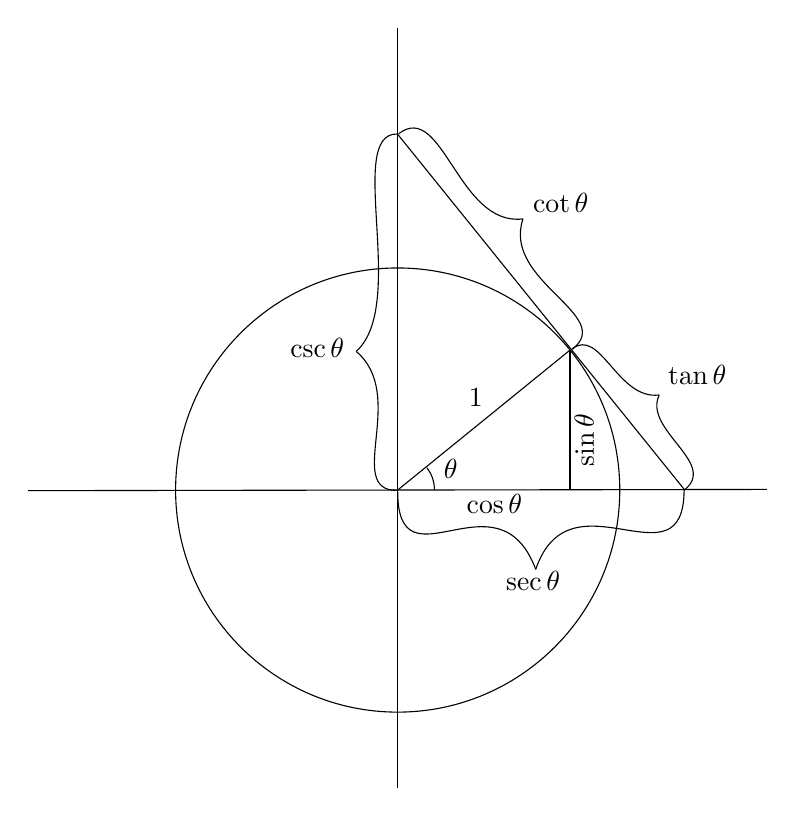
\begin{tikzpicture}[x=0.75pt,y=0.75pt,yscale=-1,xscale=1]
%uncomment if require: \path (0,434); %set diagram left start at 0, and has height of 434

%Shape: Circle [id:dp8118961016990287] 
\draw   (214,254.2) .. controls (214,195.11) and (261.91,147.2) .. (321,147.2) .. controls (380.09,147.2) and (428,195.11) .. (428,254.2) .. controls (428,313.29) and (380.09,361.2) .. (321,361.2) .. controls (261.91,361.2) and (214,313.29) .. (214,254.2) -- cycle ;
%Straight Lines [id:da6733376051381585] 
\draw    (143,254.5) -- (499,253.9) ;
%Straight Lines [id:da24708595669358502] 
\draw    (321,31.7) -- (321,397.7) ;
%Straight Lines [id:da2369525758798794] 
\draw    (404,186.8) -- (321,254.2) ;
%Straight Lines [id:da6269364989299404] 
\draw    (459,253.8) -- (321,82.8) ;
%Shape: Arc [id:dp8953631465255683] 
\draw  [draw opacity=0] (335.11,243.48) .. controls (337.38,246.45) and (338.72,250.17) .. (338.72,254.2) .. controls (338.72,254.26) and (338.72,254.32) .. (338.72,254.39) -- (321,254.2) -- cycle ; \draw   (335.11,243.48) .. controls (337.38,246.45) and (338.72,250.17) .. (338.72,254.2) .. controls (338.72,254.26) and (338.72,254.32) .. (338.72,254.39) ;  
%Straight Lines [id:da9446390224381691] 
\draw    (404,186.8) -- (404,253.8) ;
%Curve Lines [id:da6889044659660293] 
\draw    (321,254.85) .. controls (321,303.53) and (369.22,243.72) .. (387.51,292.4) ;
%Curve Lines [id:da7744827450838345] 
\draw    (387.51,292.4) .. controls (404.13,243.72) and (459,302.6) .. (459,253.92) ;
%Curve Lines [id:da7475604962570235] 
\draw    (320.73,82.66) .. controls (295.65,82.31) and (326.19,164.99) .. (301,187.4) ;
%Curve Lines [id:da536698622904964] 
\draw    (301,187.4) .. controls (325.99,208.44) and (295.33,254.05) .. (320.41,254.4) ;
%Curve Lines [id:da3819978579463683] 
\draw    (405.09,186.4) .. controls (426.34,170.03) and (371.15,153.75) .. (381.37,123.57) ;
%Curve Lines [id:da6758383716021474] 
\draw    (381.37,123.57) .. controls (350.09,127.39) and (342.7,66.17) .. (321.45,82.55) ;
%Curve Lines [id:da9285330284788131] 
\draw    (458.84,254.4) .. controls (476,241.4) and (439,225.4) .. (447,208.4) ;
%Curve Lines [id:da5181742767873634] 
\draw    (447,208.4) .. controls (426.87,210.91) and (418.68,175.48) .. (405,186.23) ;

% Text Node
\draw (342,238) node [anchor=north west][inner sep=0.75pt]    {$\theta $};
% Text Node
\draw (372,292) node [anchor=north west][inner sep=0.75pt]   [align=left] {$\displaystyle \sec \theta $};
% Text Node
\draw (268,180) node [anchor=north west][inner sep=0.75pt]   [align=left] {$\displaystyle \csc \theta $};
% Text Node
\draw (385,110) node [anchor=north west][inner sep=0.75pt]   [align=left] {$\displaystyle \cot \theta $};
% Text Node
\draw (450,193) node [anchor=north west][inner sep=0.75pt]   [align=left] {$\displaystyle \tan \theta $};
% Text Node
\draw (353,255) node [anchor=north west][inner sep=0.75pt]   [align=left] {$\displaystyle \cos \theta $};
% Text Node
\draw (405,244) node [anchor=north west][inner sep=0.75pt]  [rotate=-270] [align=left] {$\displaystyle \sin \theta $};
% Text Node
\draw (354,204) node [anchor=north west][inner sep=0.75pt]   [align=left] {$1$};


\end{tikzpicture}
}
\caption{The six common trig functions on the unit circle}
\label{6trig}
\end{figure}


To explore these functions, check out \href{https://www.desmos.com/calculator/fdr54f2jh3}{this graph on Desmos}.


\subsection{Values on the Unit Circle}

There are several angles $\theta$ for which you should be able to compute $\sin\theta$ and $\cos\theta$ (then computing the other four trig functions is easy). Luckily, there is a lot of symmetry involved: it is only necessary to memorize a few numbers and then you can easily fill in the rest.

Below is a diagram of all of the angles whose $\sin$ and $\cos$ you should be familiar with.

\begin{figure}[h!]
\label{the-unit-circle}
\centering
\fbox{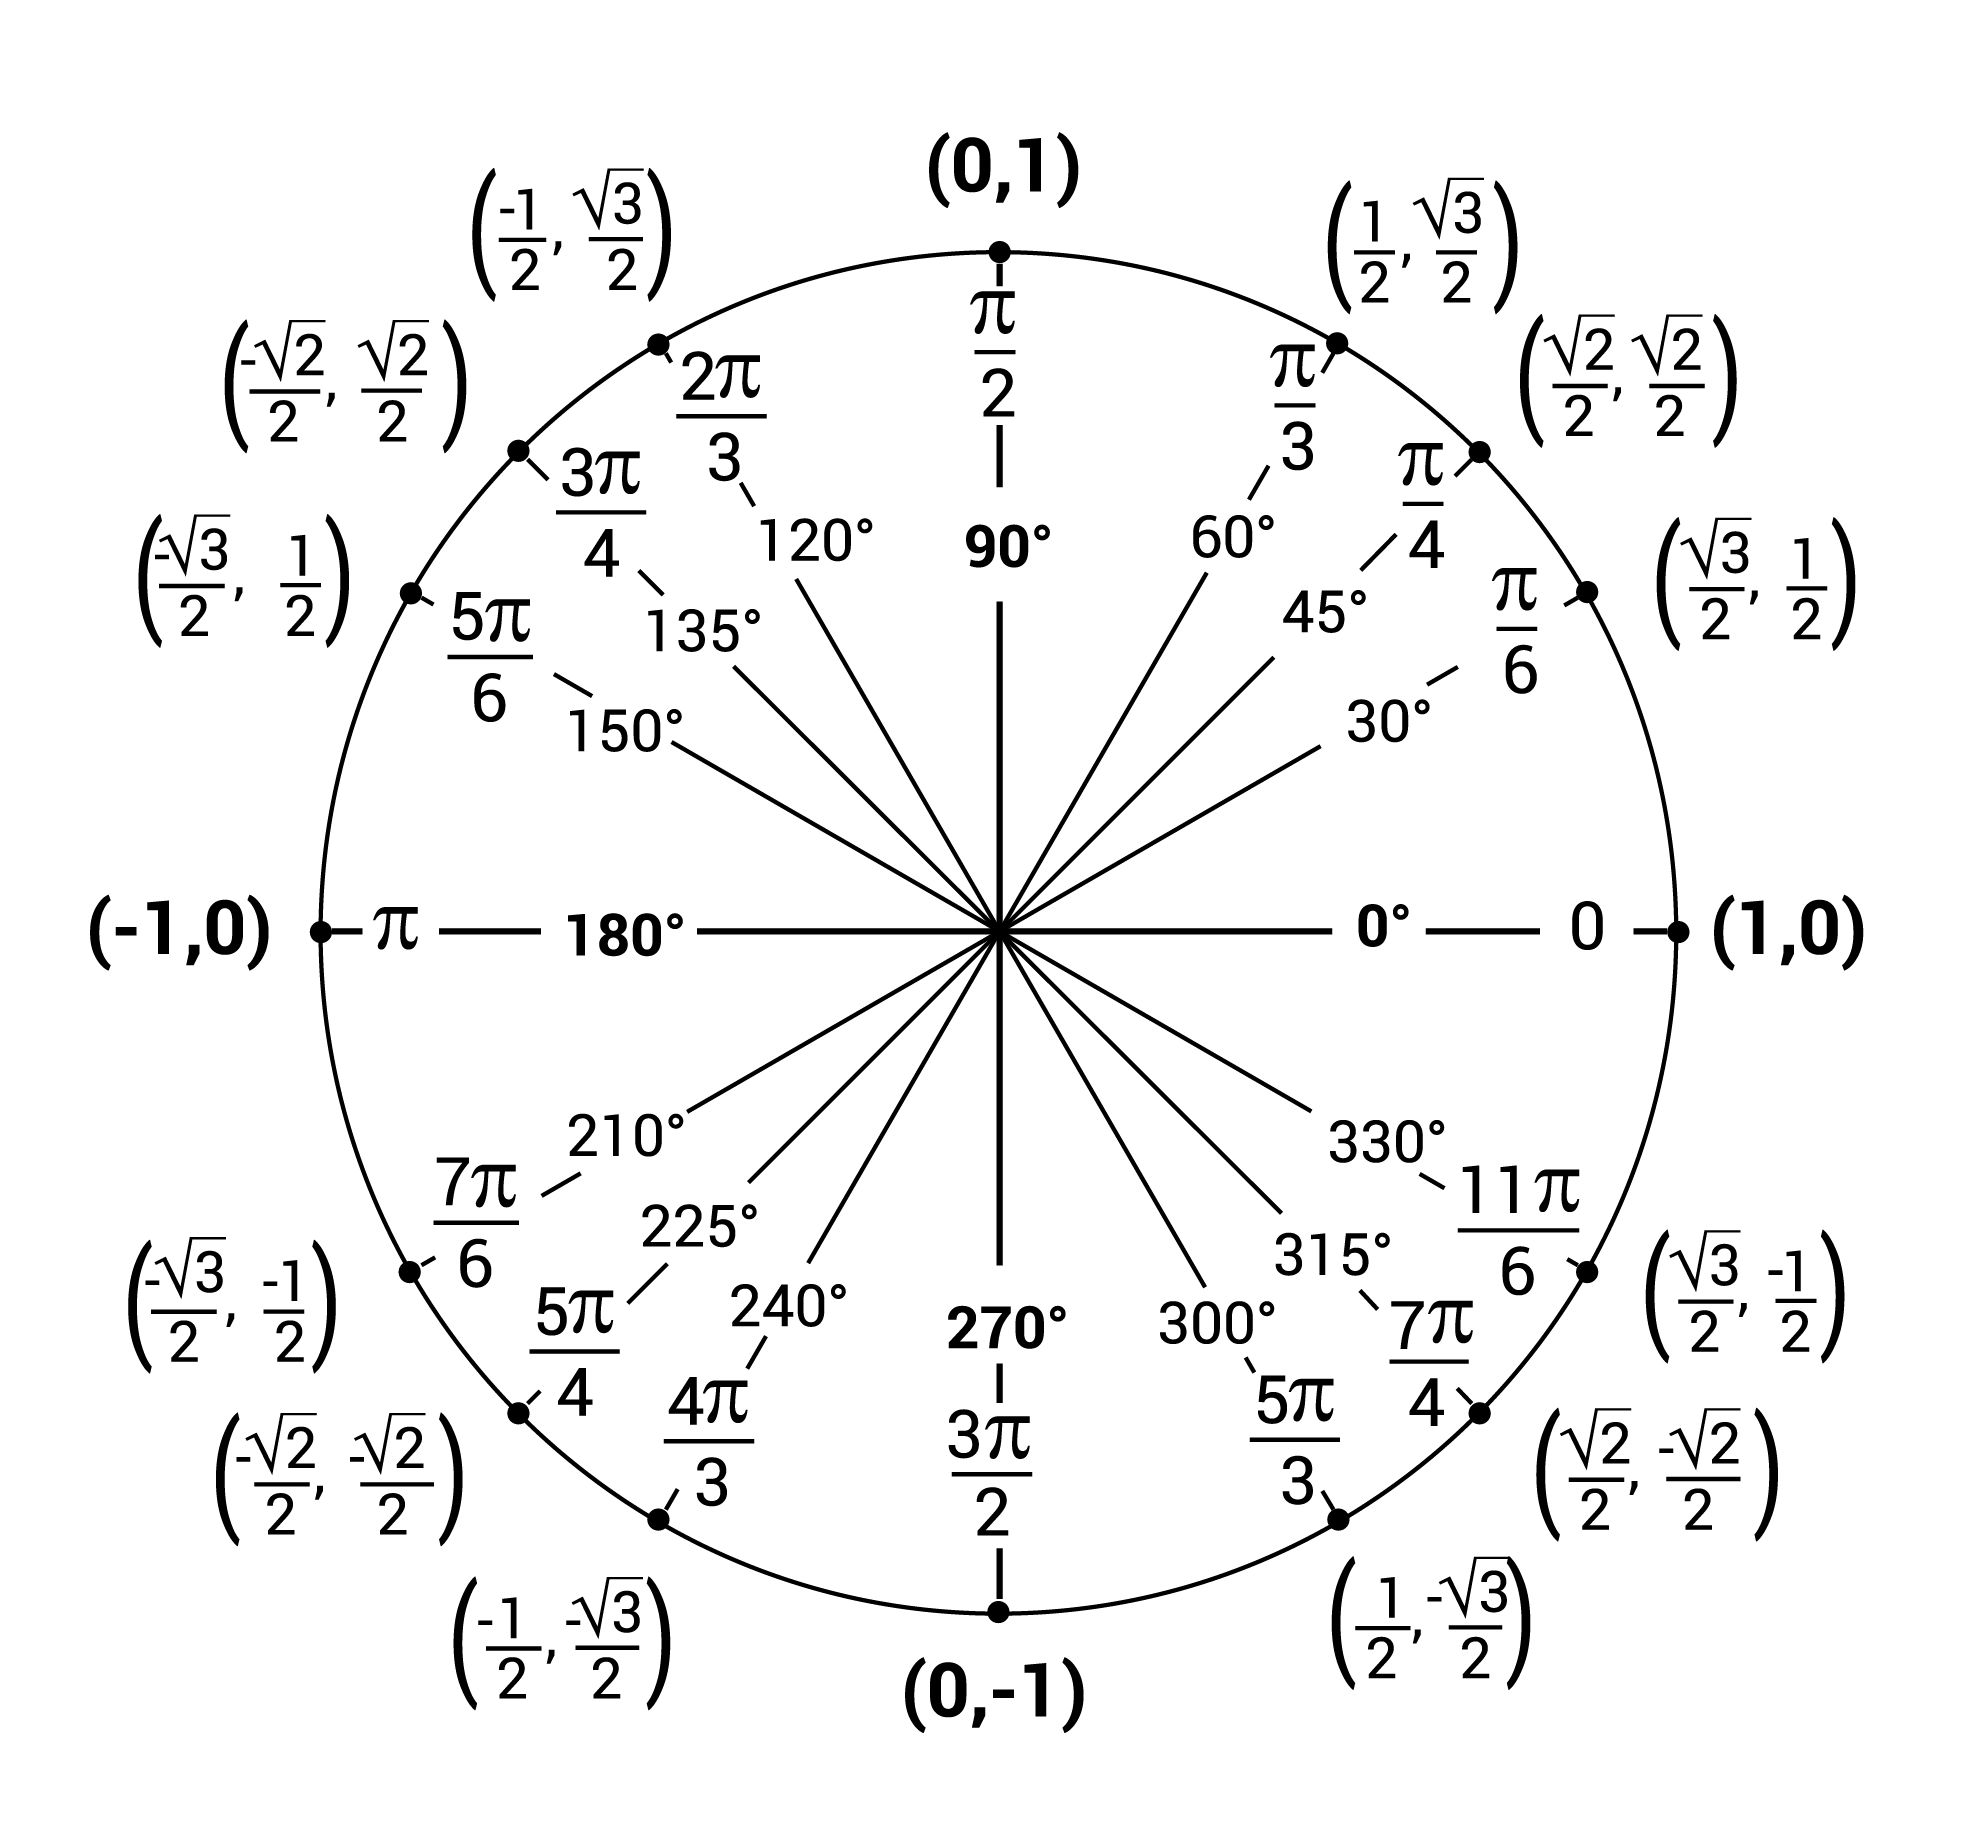
\includegraphics[width=4in]{img/unit-circle.png}}
\caption{The Unit Circle}
\end{figure}


It might seem intimidating, but just focus on the first (upper-right) quadrant and the first five angles there:


\begin{center}
\renewcommand{\arraystretch}{1.3}
\begin{tabular}{@{}lll@{}}
\toprule[0.4mm]
$\theta$ & $\cos\theta$ & $\sin\theta$ \\\midrule
   $0$  & $\sqrt{4}/2$ & $\sqrt{0}/2$ \\
$\pi/6$ & $\sqrt{3}/2$ & $\sqrt{1}/2$ \\
$\pi/4$ & $\sqrt{2}/2$ & $\sqrt{2}/2$ \\
$\pi/3$ & $\sqrt{1}/2$ & $\sqrt{3}/2$ \\
$\pi/2$ & $\sqrt{0}/2$ & $\sqrt{4}/2$ \\\bottomrule[0.4mm]
\end{tabular}
\end{center}

In this table, I wrote the numbers in an ``un-simplified'' way so you can see the pattern: their numerators change by 1 under a square-root, and as one goes up, the other goes down.

You can also see that the values for other angles are the same number, but with a different sign (according to the quadrant they are in), and that the unit circle is symmetric, reflecting over the $x$ and $y$ axis.

\subsection{The Pythagorean and Other Identities}

Remember the Pythagorean Theorem, $a^2 + b^2 = c^2$? Well, since $\sin\theta$ and $\cos\theta$ are the lengths of a right triangle with hypotenuse 1, we have the following \textbf{Pythagorean identity}:
$$\cos^2\theta +\sin^2\theta = 1.$$
\mar{Which of the following are the same?
\begin{center}
\begin{tabular}{ c c }
$\sin\theta^2$ & $\sin^2\theta$ \\
$\sin(\theta^2)$ & $\sin(\theta)^2$ \\
$(\sin(\theta))^2$ & $(\sin\theta)^2$ \\
\end{tabular}
\end{center}
}
Dividing this equation by $\sin^2\theta$ or $\cos^2\theta$, we get
$$\cot^2\theta + 1 = \csc^2\theta\quad\quad\text{and}\quad\quad 1+\tan^2\theta = \sec^2\theta.$$

There is some nice symmetry between $\sin\theta$ and $\cos\theta$. The leg opposite the angle is $\theta$ is $\sin\theta$. Since the internal angles of a triangle sum to $\pi$, the other acute angle is $\frac{\pi}{2} - \theta$. \mar{Label the angle $\frac{\pi}{2}-\theta$ on Figure \ref{sin-cos-coordinates}.} Then, the leg opposite $\frac{\pi}{2} - \theta$ has length $\sin\left(\frac{\pi}{2} - \theta\right)$, but is also $\cos\theta$. Therefore,
$$\sin\left(\frac{\pi}{2} - \theta\right) = \cos(\theta).$$
Similarly,
$$\cos\left(\frac{\pi}{2} - \theta\right) = \sin(\theta).$$
Looking at the picture of the unit circle, we can also see that
$$\sin(-\theta) = -\sin(\theta)\quad\text{and}\quad \cos(-\theta)=\cos(\theta).$$

There is one more kind of identity that will be useful for us:
$$\sin(A\pm B)=\sin A \cos B \pm \cos A \sin B,$$
$$\cos(A\pm B)=\cos A \cos B \mp \sin A \sin B.$$

These are called the \textbf{angle sum formulas}, and they are long but if you read them out loud, they make a little song! Try it while clapping on each word:
\begin{center}
``SINE-COSINE-COSINE-SINE. COSINE-COSINE-SINE-SINE.''
\end{center}\mar{No seriously, sing the song. Now do it again.}
Once you remember the order of the functions, you just have to remember that the $A$s and $B$s alternate and that the sign in the second equation flips ($\pm$ becomes $\mp$).

These simplify if $A$ and $B$ are the same angle $\theta$ to what are called the \textbf{double angle formulas}. In this case,
$$\sin(2\theta) = 2\sin\theta\cos\theta$$
and
\begin{align*}
\cos(2\theta) & = \cos^2\theta - \sin^2\theta \\
              & = 1 - 2\sin^2\theta \\
              & = 2\cos^2\theta - 1.
\end{align*}
\mar{Check that these are correct. Hint: use the Pythagorean identity.}

\subsection{Applications}

So, how do we use trigonometry to help solve problems? The main way that trigonometry is useful for you as a calculus student is two-fold. One is as a source of nice function examples to play around with (once we start taking limits and derivatives). The other is as a means to fill in missing information (this is the ``SOH-CAH-TOA'' you might remember).

Let's say you have a right triangle with hypotenuse 8 and one a $30\degree$ angle.


\begin{figure}[h!]
\centering
\tikzset{every picture/.style={line width=0.75pt}} %set default line width to 0.75pt        
\fbox{\begin{tikzpicture}[x=0.75pt,y=0.75pt,yscale=-1,xscale=1]
%uncomment if require: \path (0,300); %set diagram left start at 0, and has height of 300

%Shape: Right Triangle [id:dp06753223391248242] 
\draw   (236,78) -- (62.56,189.5) -- (236,189.5) -- cycle ;
%Shape: Arc [id:dp8301261755391214] 
\draw  [draw opacity=0] (84.77,175.15) .. controls (87.45,179.28) and (89,184.21) .. (89,189.5) -- (62.56,189.5) -- cycle ; \draw   (84.77,175.15) .. controls (87.45,179.28) and (89,184.21) .. (89,189.5) ;  
%Shape: Rectangle [id:dp7819843676440785] 
\draw   (222.88,176.38) -- (236,176.38) -- (236,189.5) -- (222.88,189.5) -- cycle ;
%Shape: Right Triangle [id:dp36110349096513206] 
\draw   (460.53,102) -- (358.65,167.49) -- (460.53,167.49) -- cycle ;
%Shape: Arc [id:dp10101111854625855] 
\draw  [draw opacity=0] (371.7,159.07) .. controls (373.27,161.49) and (374.18,164.39) .. (374.18,167.49) -- (358.65,167.49) -- cycle ; \draw   (371.7,159.07) .. controls (373.27,161.49) and (374.18,164.39) .. (374.18,167.49) ;  
%Shape: Rectangle [id:dp8285259686836064] 
\draw   (452.83,159.79) -- (460.53,159.79) -- (460.53,167.49) -- (452.83,167.49) -- cycle ;
%Curve Lines [id:da345399705785322] 
\draw    (268,78) .. controls (303.46,52.98) and (335.04,54.55) .. (366.56,76.96) ;
\draw [shift={(368,78)}, rotate = 216.18] [color={rgb, 255:red, 0; green, 0; blue, 0 }  ][line width=0.75]    (10.93,-3.29) .. controls (6.95,-1.4) and (3.31,-0.3) .. (0,0) .. controls (3.31,0.3) and (6.95,1.4) .. (10.93,3.29)   ;

% Text Node
\draw (90.25,173) node [anchor=north west][inner sep=0.75pt]    {$30\degree $};
% Text Node
\draw (136,124.4) node [anchor=north west][inner sep=0.75pt]    {$8$};
% Text Node
\draw (144,192) node [anchor=north west][inner sep=0.75pt]    {$x$};
% Text Node
\draw (238,130) node [anchor=north west][inner sep=0.75pt]    {$y$};
% Text Node
\draw (377,154) node [anchor=north west][inner sep=0.75pt]    {$30\degree $};
% Text Node
\draw (398,125) node [anchor=north west][inner sep=0.75pt]    {$1$};
% Text Node
\draw (401,169) node [anchor=north west][inner sep=0.75pt]    {$x/8$};
% Text Node
\draw (461,125) node [anchor=north west][inner sep=0.75pt]    {$y/8$};
% Text Node
\draw (301,42) node [anchor=north west][inner sep=0.75pt]    {$\div 8$};


\end{tikzpicture}}
\caption{Similar Triangles}
\end{figure}

If you want to know what the other side lengths are, this is how you can use trigonometry to do it! First, scale the triangle down by the side length that you know (in this case $8$). This doesn't change the angles, so we now have a right triangle with hypotenuse 1. By definition of $\sin$ and $\cos$,
$$\sin 30\degree = \frac{y}{8}\quad\quad\text{and}\quad\quad\cos 30\degree=\frac{x}{8},$$
so we can solve for $x$ and $y$:
$$y = 8\sin 30\degree = 4\quad\quad\text{and}\quad\quad x= 8\cos 30\degree= 4\sqrt{3}.$$
The mnemonic device ``SOH-CAH-TOA'' reminds us that \underline{S}in of $30\degree$ is the \underline{O}pposite leg ($y$) over the \underline{H}ypotenuse (8), and \underline{C}os of $30\degree$ is the \underline{A}djacent leg ($x$) over the \underline{H}ypotenuse (8). \mar{What does the ``TOA'' part say? What situation would it help you figure something out about a triangle?}

The identities that we learned about also have many applications, but mostly are in simplifying calculuations. You should keep them in mind so you recognize when they might be helpful in simplifying an expression. Here is a cool example:
\begin{align*}
\sin\left(2\theta\right)\left(\frac{\tan \theta+\cot \theta}{2}\right)
& = 2\sin\theta\cos\theta\left(\frac{\frac{\sin\theta}{\cos\theta}+\frac{\cos\theta}{\sin\theta}}{2}\right)\\
& = \sin\theta\cos\theta\left(\frac{\sin\theta}{\cos\theta}+\frac{\cos\theta}{\sin\theta}\right)\\
& = \sin^2\theta+\cos^2\theta\\
& = 1.
\end{align*}


Trig identities can also be a computationally useful tool: if you need to know the Sine (or Cosine, etc.) of an angle you are not familiar with, write the angle as a sum or difference of angles you know and use the angle sum formulas. For example,
\begin{align*}
\cos(15\degree) & = \cos(45\degree-30\degree) \\
                & = \cos(45\degree)\cos(30\degree)+\sin(45\degree)\sin(30\degree) \\
                & = \frac{\sqrt{2}}{2}\frac{\sqrt{3}}{2} + \frac{\sqrt{2}}{2}\frac{1}{2} \\
                & = \frac{\sqrt{6}+\sqrt{2}}{4}.
\end{align*}
\mar{Can you compute $\tan(75\degree)$?}

\subsection{There's Always More Trigonometry...}

Trigonometry dates back to the 3rd century BCE and needless to say it has changed a bit over the years. We've only covered the basics and focused on the trigonometry involving right triangles. There is always more trigonometry to learn: more trigonometric functions and MANY more relations among them! I won't pester you with many more right now, but they might come up in the future, so just be aware.

The two very common laws of trigonometry that involve non-right triangles are the Law of Sines and the Law of Cosines. I will state them here (for culture).

\begin{figure}[!h]
\centering
\label{circumscribed-triangle}
\tikzset{every picture/.style={line width=0.75pt}} %set default line width to 0.75pt        

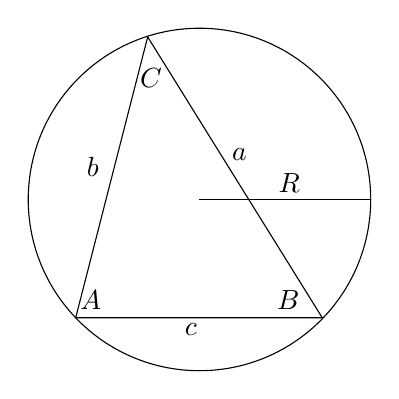
\begin{tikzpicture}[x=0.75pt,y=0.75pt,yscale=-1,xscale=1]
%uncomment if require: \path (0,476); %set diagram left start at 0, and has height of 476

%Shape: Circle [id:dp3720781821561441] 
\draw   (155,137.5) .. controls (155,91.94) and (191.94,55) .. (237.5,55) .. controls (283.06,55) and (320,91.94) .. (320,137.5) .. controls (320,183.06) and (283.06,220) .. (237.5,220) .. controls (191.94,220) and (155,183.06) .. (155,137.5) -- cycle ;
%Shape: Triangle [id:dp2721155840135763] 
\draw   (212.55,59.19) -- (296.67,194.5) -- (177.87,194.5) -- cycle ;
%Straight Lines [id:da18934326053160722] 
\draw    (237.5,137.5) -- (320,137.5) ;

% Text Node
\draw (252,111.82) node [anchor=north west][inner sep=0.75pt]    {$a$};
% Text Node
\draw (178.85,180) node [anchor=north west][inner sep=0.75pt] {$A$};
% Text Node
\draw (273.69,180) node [anchor=north west][inner sep=0.75pt] {$B$};
% Text Node
\draw (207.69,73) node [anchor=north west][inner sep=0.75pt]    {$C$};
% Text Node
\draw (229.18,196) node [anchor=north west][inner sep=0.75pt]    {$c$};
% Text Node
\draw (182,116.07) node [anchor=north west][inner sep=0.75pt]    {$b$};
% Text Node
\draw (274.32,123.82) node [anchor=north west][inner sep=0.75pt]    {$R$};


\end{tikzpicture}
\caption{Circumscribed Triangle}
\end{figure}

Figure \ref{circumscribed-triangle} shows a triangle with internal angles $A$, $B$, and $C$, and respective opposite side lengths $a$, $b$, and $c$. The triangle is \textbf{circumscribed} in a circle, meaning its vertices lie on the circle's boundary. It turns out that the circle has radius
$$R=\frac{abc}{\sqrt{(a+b+c)(a-b+c)(a+b-c)(-a+b+c)}}.$$



\begin{theorem}[Law of Sines]
If a triangle has sides and angles as above, then
$$\frac{a}{\sin A}=\frac{b}{\sin B}=\frac{c}{\sin C}=2R=\frac{abc}{2\Delta},$$
where $R$ is the radius of the circumscribed circle and $\Delta$ is the area of the triangle.
\end{theorem}

\begin{theorem}[Law of Cosines]
If a triangle has sides and angles as above, then
$$a^2+b^2=c^2+2ab\cos C.$$
\end{theorem}
\mar{Almost looks familiar, doesn't it?}

When you use these formulas, keep in mind that solving for an angle can be tricky: if $\sin\theta=1/2$, then $\theta$ could be $30\degree$, $150\degree$, $390\degree$, etc..



\section{Functions on the Real Line}

\subsection{Real Numbers}

The set of real numbers ($\R$) is an uncountably infinite set, meaning I can not even begin to exhaustively list all of its members. However, here are some of my favorites: $3$, $2/5$, $4.11$, $713$, $\sqrt{37}$, $\pi$. Real numbers include both the rationals and irrationals. \mar{Do you know any numbers that aren't real?}

The real numbers can be thought of as a continuum that has no beginning and no end: real numbers can get infinitely small and infinitely large.

More concretely, imagine you are standing on a road that goes on forever, both in front of you and behind you. If you drop a traffic cone where you are standing, and call it ``the origin'', then any distance you walk on this road away from the cone is a real number. If you walk forward, it is positive, and if you walk backwards, it is negative. You can keep walking forever and reach any number you would like, but you will never reach an ``end of the road'' because it doesn't exist.

\subsection{Subsets of the Real Line}

A \textbf{subset} is a subcollection. There are a few ways we notate subsets of $\R$, so this section is mostly dedicated to notation. The first two examples of a subset are kind of stupid: the \textbf{empty set} $\emptyset$ (the set with no elements), and all of $\R$ are both subsets of $\R$.

You can define a \textbf{literal} subset of $\R$ by listing the elements it contains. For example, $\{1,2,3\}$ is the set containing 1, 2, and 3.

\textbf{Intervals} are---in my opinion---the most important kind of subset of $\R$. The following table shows the 8 kinds of intervals and the two ways we write them ($a\leq b$ are real numbers).

\begin{center}
\renewcommand{\arraystretch}{1.1}
\begin{tabular}{p{3.5in} p{1.25in} p{1.3in}}
\toprule[0.4mm]
The set of real numbers that are... & \textbf{Interval Notation} & \textbf{Set-Builder Notation} \\ \midrule
greater than $a$ and less than $b$ & $(a,b)$ & $\{x\in\R\ :\ a < x < b\}$ \\
greater than or equal to $a$ and less than $b$ & $[a,b)$ & $\{x\in\R\ :\ a \leq x < b\}$ \\
greater than $a$ and less than or equal to $b$ & $(a,b]$ & $\{x\in\R\ :\ a < x \leq b\}$ \\
greater than or equal to $a$ and less than or equal to $b$ & $[a,b]$ & $\{x\in\R\ :\ a \leq x \leq b\}$ \\
greater than $a$ & $(a,\infty)$ & $\{x\in\R\ :\ a < x\}$ \\
greater than or equal to $a$ & $[a,\infty)$ & $\{x\in\R\ :\ a \leq x\}$ \\
less than $b$ & $(-\infty,b)$ & $\{x\in\R\ :\ x < b\}$ \\
less than or equal to $b$ & $(-\infty,b]$ & $\{x\in\R\ :\ x \leq b\}$ \\
\bottomrule
\end{tabular}
\end{center}


Interval notation is easy to write and read, once you get a hang of what the different parentheses mean. The regular parentheses $()$ are called ``open'' and mean that the particular endpoint of the interval is not included. The $[]$ brackets are called ``closed'' and indicate that the endpoint \textit{is} included. \mar{Why aren't $(a,\infty]$, $(a,\infty]$, $[-\infty,b)$, and $[-\infty,b]$ included in the table?}

The set-builder notation is read as follows:

% \vspace*{1em}

\begin{Large}
$$\{\underbrace{x}_x\underbrace{\in}_\text{in}\underbrace{\R}_{\text{the real}\atop \text{numbers}}\ \underbrace{:}_\text{such that}\ \underbrace{a < x < b}_{x\text{ is strictly}\atop\text{between }a\text{ and }b}}\}.$$
\end{Large}

% \vspace*{1em}


All of the subsets of $\R$ that you'll want to use in this course can be written using combinations of intervals. There are two ways to do this:
\begin{itemize}
\item The \textbf{union} of two sets is the set that contains all of the elements in either set and is denoted with the ``cup'' symbol, $\cup$. Here are some examples:
\begin{enumerate}
\item $\{1, 2, 3\}\cup\{3, 4, 5\} = \{1,2,3,4,5\}$
\item $(3,4]\cup[4,5) = (3,5)$
\item $(-\infty,5)\cup[5,\infty) = (-\infty,\infty)=\R$
\item $(-3,0)\cup(2,6)$
\item $(1,5)\cup(3, 7) = (1,7)$
\item $(1,8)\cup(3, 4) = (1,8)$
\end{enumerate}
\item The \textbf{intersection} of two sets is the set that contains the elements in both sets and is denoted with the ``cap'' symbol, $\cap$. Here are some examples:
\begin{enumerate}
\item $\{1, 2, 3\}\cap\{3, 4, 5\} = \{3\}$
\item $(3,4]\cap[4,5) = \{4\}$
\item $(-\infty,5)\cap[5,\infty) = \emptyset$
\item $(-3,0)\cap(2,6)=\emptyset$
\item $(1,5)\cap(3, 7) = (3,5)$
\item $(1,8)\cap(3,4) = (3,4)$
\end{enumerate}
\end{itemize}

\mar{Draw a picture of each of these examples. Does \textit{Venn diagram} ring any bells?}

\subsection{Defining Functions}

We will start with quite a few new (and abstract) definitions, but we will make things concrete very soon.

If $A$ and $B$ are two sets, a \textbf{function} $f$ from $A$ to $B$ is an assignment of each element of $A$ to a unique element of $B$. In other words, for each input $a$ in $A$, $f$ outputs exactly one $b$ in $B$, which we denote as $f(a)$. The set $A$ is called the \textbf{domain} of $f$, the set $B$ is called the \textbf{codomain} of $f$, and we write $$f:A\to B\quad\quad\text{ or }\quad\quad A\overset{f}{\to} B.$$
Please remember that a function has three pieces of information: the domain, the codomain, and the rule of assignment. If one of these pieces is changed, the resulting function is different. \mar{Is $f$ defined by $$f(x)=\begin{cases}x+1 & x > 0 \\ x^2 & x < 1\end{cases}$$ a function?}

The \textbf{range} of $f$ is the set of all outputs of $f$ and is denoted $f(A)$. The range is always a subset of the codomain, but they are not always equal sets. The relationship between the domain, codomain, and the range are an important one:
\begin{itemize}
\item A function is called \textbf{surjective} (or \textbf{onto}) if its range and codomain are the same (i.e. $f(A)=B$). In other words, a function is surjective if every element of the codomain is an output of $f$. \mar{What does the word ``sur'' mean in French?}
\item A function is called \textbf{injective} (or \textbf{one-to-one}) if each element of the range is the output of exactly one element of the domain. In other words, if $f(x_1)=f(x_2)$, then $x_1=x_2$.
\item If a function is both surjective and injective, then it is called \textbf{bijective}.
\end{itemize}

The figure below is a cartoon of three functions. From left to right, (1) a surjection that is not injective, (2) a bijection, and (3) an injection that is not surjective. \mar{Write down the domain, codomain, and range of each of these functions.}



\begin{figure}[H]
\label{three-functions}
\centering
\fbox{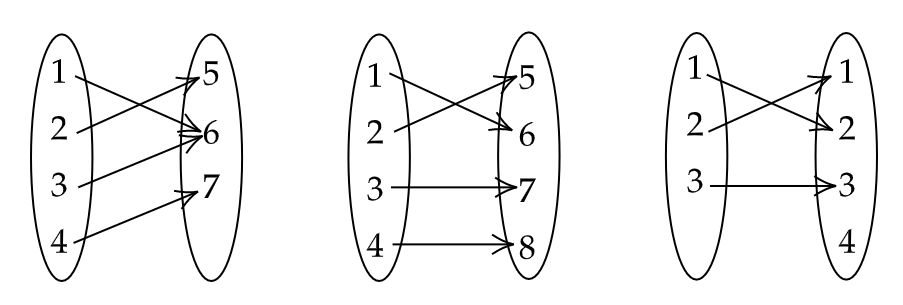
\includegraphics[width=4in]{img/three-functions.png}}
\caption{A Surjection, a Bijection, and an Injection}
\end{figure}


We will only use \textbf{real functions}, which are functions whose domain and codomain are subsets of $\R$. These functions take real numbers as inputs and give real numbers as outputs, so they can be graphed on a Cartesian grid, with the inputs on the horizontal axis and outputs on the vertical axis.

To check that a curve drawn on a plot is a function, you can use the \textbf{vertical line test}: \mar{Draw a non-function that fails the vertical line test.} any vertical line must intersect a graph of a real function at most once (i.e. if a vertical line intersects a curve more than once, then the curve cannot be the graph of a real function).


Some people may get sloppy and say things like
\begin{center}
``the function $f(x)=x^2$''
\end{center}
but what they really mean is
\begin{center}
``the real function $f$, defined by $f(x)=x^2$''.
\end{center}
Distinguishing between a function and the formula defining it will eventually make things easier to understand. However, from now on, I might say ``function'' and mean ``real-function'' (use context clues). \mar{Think of real functions that are (1) injective but not surjective, (2) surjective but not injective, (3) neither injective nor surjective, (4) bijective.}


\subsection{More Domains and Ranges}

All real functions can have $\R$ as their codomain, but not all real functions have $\R$ as their domain and range. The following table lists domains and ranges for some common functions.

\begin{center}
\renewcommand{\arraystretch}{1.3}
\begin{tabular}{@{}p{1in}p{1.6in}lp{2.25in}@{}}
\toprule[0.4mm]
Function type & & Domain & Range \\
\hline
Polynomial & $a_nx^n+\cdots+a_1x+a_0$ & $\R$ & If the highest power is odd, $\R$. If the highest power is even and positive, then $[b,\infty)$, and $(-\infty,b)$ otherwise (for some $b$).\\
Exponential & $a^x$ & $\R$ & $(0,\infty)$\\
Logarithm & $\log_a(x)$ & $(0,\infty)$ & $\R$\\
Rational & $\frac{p(x)}{q(x)}$ \hspace{3in} ($p$, $q$ are polynomials) & $\{x\in\R\ :\ q(x)\neq 0\}$ & It depends\\
\bottomrule[0.4mm]
\end{tabular}
\end{center}



Let's do some concrete examples:
\begin{itemize}
\item The function $f$ given by $f(x)=\frac{1}{x}$ does not have 0 in its domain, since we can't divide by 0. Also, $f$ does not have 0 in its range, since there is no real number $x$ for which $\frac{1}{x}=0$. Therefore the domain and range of $f$ are both $(-\infty,0)\cup(0,\infty)$.
\item Similarly, $\tan$ does not have $2n\pi+\pi/2$ in its domain for any integer $n$, since $\cos(2n\pi+\pi/2)=0$ (we can write the domain of $\tan$ as $\{x\in\R\ :\ x\neq 2n\pi + \pi/2\text{ for any integer }n\}$).  The range of $\tan$ is all of $\R$.
\item The function $f$ given by $f(x)=x^2$ has domain $\R$ and range $[0,\infty)$. \mar{What is the domain and range of $f$ given by $f(x)=n^n$ where $n$ is a positive integer ($n=1, 2, 3, \dots$)?}
\end{itemize}





\subsection{Inverses}
A function $f:A\to B$ is \textbf{invertible} if there is some function $g:B\to A$ such that two conditions hold:
\begin{enumerate}
\item[(i)] for all $a$ in $A$, $g(f(a))=a$;
\item[(ii)] for all $b$ in $B$, $f(g(b))=b$.
\end{enumerate}
In this case, we call $g$ the \textbf{inverse} of $f$ and write $f^{-1}=g$. In other words, a function is \textbf{invertible} if it is reversible as a mapping: if $f$ maps $x$ to $y:=f(x)$, then its inverse $f^{-1}$ must map $y$ to $x$. \mar{Look abck at Figure \ref{three-functions}. Which of these functions are invertible? On any function that is invertible, draw the arrows for the inverse function.}

You might wonder: \textit{when is a function invertible?} It turns out that we already understand exactly what we want:
\begin{thm}
A function is invertible exactly when it is bijective.
\end{thm}
Lets think through this: looking back at Figure \ref{three-functions}, the first function is not invertible because it is not injective. Both 1 and 3 map to 6, but condition (i) says that we must have $f^{-1}(f(1))=1$ and $f^{-1}(f(3))=3$. Since $f(1)$ and $f(3)$ are both equal to $6$, we must have that $1=f^{-1}(6)=3$, crazy talk!

The third function in Figure \ref{three-functions} is not invertible because it is not surjective. This is a problem: since the element 4 in the codomain is not mapped to by eny element of the domain, no matter what we might chose $f^{-1}(4)$ to be, $f(f^{-1}(4))\neq 4$, which violates condition (ii).

The condition that invertible functions must be injective is sometimes called the \textbf{horizontal line test} for real functions: the graph of an invertible real function cannot intersect any horizontal line more than once (i.e. if a horizontal line intersects the graph of a function more than once, then the function cannot be invertible). \mar{Draw the graph of a non-invertible function failing the horizontal line test.}

The general strategy for finding a functions inverse is to switch the place of $x$ and $y$ in the equation, and then solve for $y$. The result, if it exists, will give you an inverse for the original function (on a possibly smaller domain). Graphically, the inverse of a function is a reflection of the function across the line $y=x$. If a function is not bijective, we can ``fix'' it by making its domain or codomain smaller. For any function there are several ways to do this, but there are some agreed upon conventions that I'll outline below.

\begin{itemize}
\item The function $f$ defined by $f(x)=x^2$ has domain $\R$, but is not invertible: the line $y=4$ intersects the graph in two places, $(-2,4)$ and $(2,4)$. However, we can can change both its domain and codomain to be $[0,\infty)$. To find its inverse, solve the equation $x=y^2$ for $y$. We get $y=\pm\sqrt{x}$, but since we are changing the domain of $f$ to only the non-negative real numbers, we forget about the negative square root. Then the inverse of $f$ is given by $f^{-1}=\sqrt{x}$, and for any non-negative $x$ and $y$ ($x,y\in[0,\infty)$),
$$f^{-1}(f(y))=f(x^2)=\sqrt{(x)^2})=x$$
and
$$f(f^{-1}(y))=f(\sqrt{y})=(\sqrt{y})^2=y.$$
\item The function $\sin$ has domain $\R$ and range $[-1,1]$ but is \textbf{periodic} (meaning its values cyclically repeat) so cannot be invertible without an adjustment to its domain. The smaller domain we choose is $[-\pi/2,\pi/2]$ and the modified codomain is its range, $[-1,1]$. The inverse of $\sin$ is called $\arcsin$ or $\sin^{-1}$ and has domain $[-1,1]$ and range $[-\pi/2,\pi/2]$. \mar{Look up the modified domains and codomains for the other inverse trig functions.}
\item The function $f(x)=e^x$ has domain $\R$ and range $(0,\infty)$. If we shrink the codomain $\R$ to be equal to the range, then its inverse is given by $f^{-f}(x)=\ln(x)$ and domain $(0,\infty)$ and range $\R$.
\end{itemize}








\newpage
\part{Limits and Continuity}

\section{Limits}

Limits are important in calculus since we need very small quantities to effectively study change. Yeah, that's pretty vague, but hopefully it'll clear up in a few pages.

We study limits for many reasons. One of them is to study functions at points where they are only ``close'' to being defined. For example, the function $f$ given by $f(x)=\frac{x(x+1)}{x}$ is not defined at $0$, but looks like the line $x+1$ everywhere else.

\subsection{Intuitive Limits}

The intuitive idea of a \textbf{limit} is to examine what the output of a function does as the input moves close to a specific value. Since the functions we care about take real numbers as inputs, there are two ways you can approach a number on the real line (from the left and from the right). We will talk about left- and right-sided limits.

Before getting into the actual definition, we'll start intuitively. If a function is     ``continuous''\footnote{I put this word in quotes because I haven't defined it yet, but you should have an intuitive idea of what this means: being able to draw it without lifting your pencil. Just wait for a few pages.} and is defined at $a$, then as $x$ moves closer to $a$, $f(x)$ moves closer to $f(a)$, so the limit of $f$ as $x$ approaches $a$ is $f(a)$.


Let's get a little more general: suppose a function $f$ is defined on open intervals on either side of $a$.

If $f$ is defined on an interval to the \textit{left} of $a$ and the values of $f(x)$ approach $L$ as $x$ approaches $a$ from the \textit{left}, we say that the ``\textbf{left-sided limit of $f$ as $x$ approaches $a$} is $L$'' and we write $$\lim_{x\to a^-}f(x)=L.$$
If $f$ is defined on an interval to the \textit{right} of $a$ and the values of $f(x)$ approach $L$ as $x$ approaches $a$ from the \textit{right}, we say that the \textbf{right-sided limit of $f$ as $x$ approaches $a$} is $L$'' and we write
$$\lim_{x\to a^+}f(x)=L.$$
If the right and left sided limits match, then we say that the \textbf{limit of $f$ as $x$ approaches $a$ is $L$} and write $$\lim_{x\to a}f(x)=L.$$

\noindent Note: $f$ need not be defined at $a$ to find the limit of $f$ as $x$ approaches $a$.

\vspace{1em}

One can compute $f(x)$ for values of $x$ that get closer and closer to either side of $a$. If the values approach $L$, then you have good reason to believe that $L$ is the (right- and/or left-sided) limit.

\begin{center}
\begin{tabular}{@{}ll@{}}
\toprule[0.4mm]
   $x$        & $f(x)$        \\
\midrule
   $a-0.1$    & $f(a-0.1)$    \\
   $a-0.01$   & $f(a-0.01)$   \\
   $a-0.001$  & $f(a-0.001)$  \\
   $a-0.0001$ & $f(a-0.0001)$ \\
\midrule
   $a+0.0001$ & $f(a+0.0001)$ \\
   $a+0.001$  & $f(a+0.001)$  \\
   $a+0.01$   & $f(a+0.01)$   \\
   $a+0.1$    & $f(a+0.1)$    \\
\bottomrule[0.4mm]
\end{tabular}
\end{center}

Such calculations, however, cannot prove that a function limits to a specific value.

\subsection{Infinite Limits}

We can extend the idea of limits outside of the real numbers to include positive and negative infinity in place of both $a$ and $L$.
\begin{itemize}
\item If $f(x)$ grows without bound as $x$ approaches $a$ from the left, then we write $$\lim_{x\to a^-}f(x)=\infty.$$
(Similarly for $x$ approaching $a$ from the right, and also if $f(x)$ becomes increasingly negative without bound).
\item We denote the value (if such a value exists) that $f(x)$ approaches as $x$ approaches $\infty$ as $$\lim_{x\to\infty} f(x).$$
(Similarly if $x$ approaches $-\infty$).
\end{itemize}



\subsection{Optional: The $\varepsilon-\delta$ Definition}

You may be dissatisfied with the intuitive approach to limits, so we can make the definition more rigorous. The main idea that needs to be captured by a formal definition is \textit{arbitrary precision}. That is, we need a way to say formally that ``$f(x)$ approaches $L$ as $x$ approaches $a$.''

By controlling the input $x$, we must be able to make the distance $|f(x)-L|$ between the output $f(x)$ and $L$ to be as small as we want (``arbitrarily small''). In other words, if $\varepsilon>0$ is any small positive number, we must be able to ensure (by controlling $x$) that $|f(x)-L| < \varepsilon$. To control $x$, we can make the distance $|x-a|$ between $x$ and $a$ smaller than some positive number $\delta > 0$ (that may depend on $\varepsilon$).

Now we're ready for the real ``$\varepsilon-\delta$'' definition of a limit: we say that \textbf{$L$ is the limit of $f$ as $x$ approaches $a$} if
$$\text{for all } \varepsilon > 0, \text{ there is some } \delta > 0, \text{ such that } |x - a| < \delta \implies |f(x) - L| <\varepsilon.$$

Read that last line a few times, because statements with multiple quantifiers can be tricky!

\begin{figure}[h!]
\centering
\fbox{
\tikzset{every picture/.style={line width=0.75pt}}
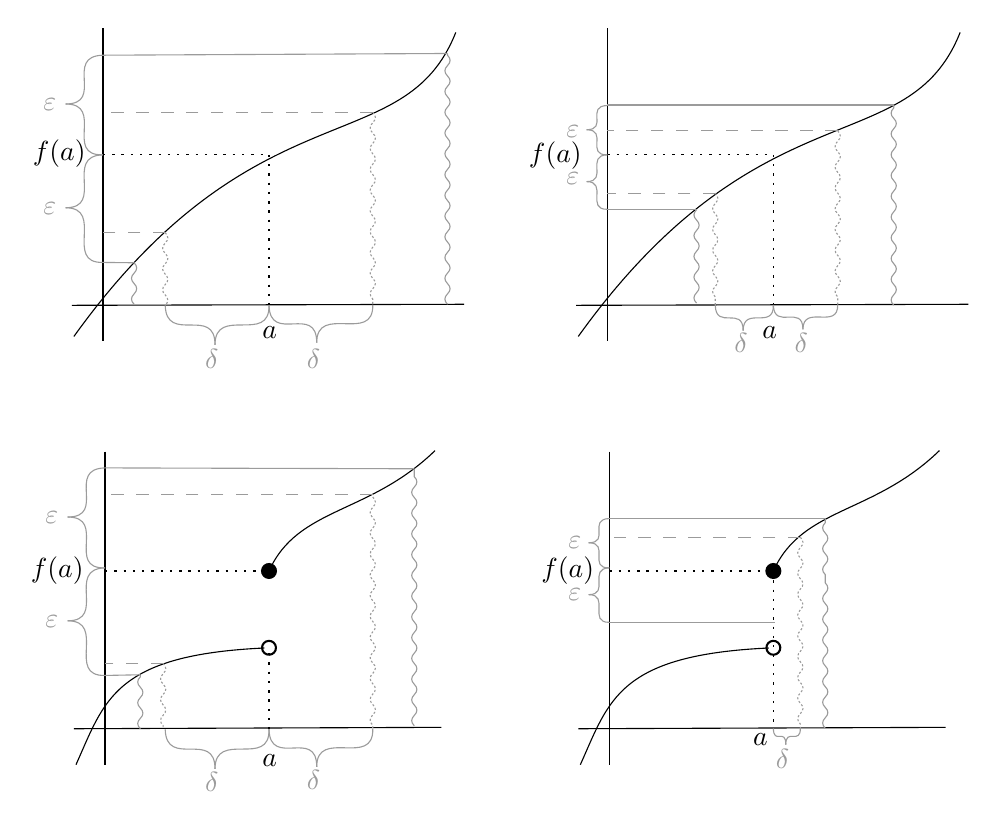
\begin{tikzpicture}[x=0.75pt,y=0.75pt,yscale=-1,xscale=1]
%uncomment if require: \path (0,428); %set diagram left start at 0, and has height of 428

%Straight Lines [id:da2730924968926851] 
\draw    (71,155) -- (260,154.5) ;
%Straight Lines [id:da38663844155403493] 
\draw    (86,21.5) -- (86,172.33) ;
%Curve Lines [id:da5832897062677318] 
\draw    (72,170) .. controls (160,47.5) and (231,86.5) .. (256,23.5) ;
%Curve Lines [id:da15926967534570857] 
\draw    (73,376.33) .. controls (86.86,345.64) and (90.92,323.45) .. (163.77,320.1) ;
\draw [shift={(166,320)}, rotate = 357.71] [color={rgb, 255:red, 0; green, 0; blue, 0 }  ][line width=0.75]      (0, 0) circle [x radius= 3.35, y radius= 3.35]   ;
%Curve Lines [id:da573129079856388] 
\draw    (166,283) .. controls (180,252) and (214,256) .. (246,225) ;
\draw [shift={(166,283)}, rotate = 294.3] [color={rgb, 255:red, 0; green, 0; blue, 0 }  ][fill={rgb, 255:red, 0; green, 0; blue, 0 }  ][line width=0.75]      (0, 0) circle [x radius= 3.35, y radius= 3.35]   ;
%Straight Lines [id:da06544192635535961] 
\draw  [dash pattern={on 0.84pt off 2.51pt}]  (166,82.5) -- (166,154.92) ;
%Straight Lines [id:da8462520068785757] 
\draw  [dash pattern={on 0.84pt off 2.51pt}]  (86,82.5) -- (166,82.5) ;
%Straight Lines [id:da8033956316212987] 
\draw [color={rgb, 255:red, 155; green, 155; blue, 155 }  ,draw opacity=1 ]   (86,34.5) -- (252,33.67) ;
%Straight Lines [id:da9058328806059841] 
\draw [color={rgb, 255:red, 155; green, 155; blue, 155 }  ,draw opacity=1 ]   (86,134.33) -- (101,134.5) ;
%Straight Lines [id:da7683874289412185] 
\draw    (72,359) -- (249,358.33) ;
%Straight Lines [id:da21021021460529377] 
\draw    (87,225.5) -- (87,376.33) ;
%Straight Lines [id:da5263630709862186] 
\draw  [dash pattern={on 0.84pt off 2.51pt}]  (166,322.58) -- (166,359.25) ;
%Straight Lines [id:da2255352189878881] 
\draw  [dash pattern={on 0.84pt off 2.51pt}]  (87,283) -- (166,283) ;
%Straight Lines [id:da12241776303117424] 
\draw [color={rgb, 255:red, 155; green, 155; blue, 155 }  ,draw opacity=1 ]   (87,233.33) -- (236,233.75) ;
%Straight Lines [id:da6551551228954233] 
\draw [color={rgb, 255:red, 155; green, 155; blue, 155 }  ,draw opacity=1 ]   (87,333.33) -- (104,333) ;
%Straight Lines [id:da3470258564776276] 
\draw [color={rgb, 255:red, 155; green, 155; blue, 155 }  ,draw opacity=1 ] [dash pattern={on 0.75pt off 0.75pt}]  (116,120) .. controls (117.67,121.67) and (117.67,123.33) .. (116,125) .. controls (114.33,126.67) and (114.33,128.33) .. (116,130) .. controls (117.67,131.67) and (117.67,133.33) .. (116,135) .. controls (114.33,136.67) and (114.33,138.33) .. (116,140) .. controls (117.67,141.67) and (117.67,143.33) .. (116,145) .. controls (114.33,146.67) and (114.33,148.33) .. (116,150) .. controls (117.67,151.67) and (117.67,153.33) .. (116,155) -- (116,155) ;
%Straight Lines [id:da2371091562631653] 
\draw [color={rgb, 255:red, 155; green, 155; blue, 155 }  ,draw opacity=1 ] [dash pattern={on 0.75pt off 0.75pt}]  (216,62) .. controls (217.67,63.67) and (217.67,65.33) .. (216,67) .. controls (214.33,68.67) and (214.33,70.33) .. (216,72) .. controls (217.67,73.67) and (217.67,75.33) .. (216,77) .. controls (214.33,78.67) and (214.33,80.33) .. (216,82) .. controls (217.67,83.67) and (217.67,85.33) .. (216,87) .. controls (214.33,88.67) and (214.33,90.33) .. (216,92) .. controls (217.67,93.67) and (217.67,95.33) .. (216,97) .. controls (214.33,98.67) and (214.33,100.33) .. (216,102) .. controls (217.67,103.67) and (217.67,105.33) .. (216,107) .. controls (214.33,108.67) and (214.33,110.33) .. (216,112) .. controls (217.67,113.67) and (217.67,115.33) .. (216,117) .. controls (214.33,118.67) and (214.33,120.33) .. (216,122) .. controls (217.67,123.67) and (217.67,125.33) .. (216,127) .. controls (214.33,128.67) and (214.33,130.33) .. (216,132) .. controls (217.67,133.67) and (217.67,135.33) .. (216,137) .. controls (214.33,138.67) and (214.33,140.33) .. (216,142) .. controls (217.67,143.67) and (217.67,145.33) .. (216,147) .. controls (214.33,148.67) and (214.33,150.33) .. (216,152) -- (216,154.71) -- (216,154.71) ;
%Straight Lines [id:da47940446384008517] 
\draw [color={rgb, 255:red, 155; green, 155; blue, 155 }  ,draw opacity=1 ] [dash pattern={on 4.5pt off 4.5pt}]  (116,120) -- (86,120) ;
%Straight Lines [id:da2718218581855085] 
\draw [color={rgb, 255:red, 155; green, 155; blue, 155 }  ,draw opacity=1 ] [dash pattern={on 4.5pt off 4.5pt}]  (216,62) -- (86,62) ;
%Curve Lines [id:da7867325499156288] 
\draw [color={rgb, 255:red, 155; green, 155; blue, 155 }  ,draw opacity=1 ]   (68,58) .. controls (87,58) and (67,35) .. (86,34.5) ;
%Curve Lines [id:da8389021578247982] 
\draw [color={rgb, 255:red, 155; green, 155; blue, 155 }  ,draw opacity=1 ]   (68,58) .. controls (87,58) and (67,83) .. (86,82.5) ;
%Curve Lines [id:da6940267896547274] 
\draw [color={rgb, 255:red, 155; green, 155; blue, 155 }  ,draw opacity=1 ]   (68,108) .. controls (87,108) and (67,83) .. (86,82.5) ;
%Curve Lines [id:da9368251006708403] 
\draw [color={rgb, 255:red, 155; green, 155; blue, 155 }  ,draw opacity=1 ]   (68,108) .. controls (87,108) and (67,134.83) .. (86,134.33) ;
%Curve Lines [id:da7416463958304471] 
\draw [color={rgb, 255:red, 155; green, 155; blue, 155 }  ,draw opacity=1 ]   (139.99,174) .. controls (140,155) and (116.5,174) .. (116,155) ;
%Curve Lines [id:da0946019041451891] 
\draw [color={rgb, 255:red, 155; green, 155; blue, 155 }  ,draw opacity=1 ]   (139.99,174) .. controls (140,155) and (166.5,173.92) .. (166,154.92) ;
%Curve Lines [id:da8479225025412045] 
\draw [color={rgb, 255:red, 155; green, 155; blue, 155 }  ,draw opacity=1 ]   (188.99,173) .. controls (189,154) and (166.5,173.92) .. (166,154.92) ;
%Curve Lines [id:da5287374586288269] 
\draw [color={rgb, 255:red, 155; green, 155; blue, 155 }  ,draw opacity=1 ]   (188.99,173) .. controls (189,154) and (216.5,173.71) .. (216,154.71) ;
%Straight Lines [id:da5763369512697336] 
\draw [color={rgb, 255:red, 155; green, 155; blue, 155 }  ,draw opacity=1 ]   (101,154.5) .. controls (99.33,152.83) and (99.33,151.17) .. (101,149.5) .. controls (102.67,147.83) and (102.67,146.17) .. (101,144.5) .. controls (99.33,142.83) and (99.33,141.17) .. (101,139.5) .. controls (102.67,137.83) and (102.67,136.17) .. (101,134.5) -- (101,134.5) ;
%Straight Lines [id:da9925497456851824] 
\draw [color={rgb, 255:red, 155; green, 155; blue, 155 }  ,draw opacity=1 ]   (252,154.5) .. controls (250.33,152.83) and (250.33,151.17) .. (252,149.5) .. controls (253.67,147.83) and (253.67,146.17) .. (252,144.5) .. controls (250.33,142.83) and (250.33,141.17) .. (252,139.5) .. controls (253.67,137.83) and (253.67,136.17) .. (252,134.5) .. controls (250.33,132.83) and (250.33,131.17) .. (252,129.5) .. controls (253.67,127.83) and (253.67,126.17) .. (252,124.5) .. controls (250.33,122.83) and (250.33,121.17) .. (252,119.5) .. controls (253.67,117.83) and (253.67,116.17) .. (252,114.5) .. controls (250.33,112.83) and (250.33,111.17) .. (252,109.5) .. controls (253.67,107.83) and (253.67,106.17) .. (252,104.5) .. controls (250.33,102.83) and (250.33,101.17) .. (252,99.5) .. controls (253.67,97.83) and (253.67,96.17) .. (252,94.5) .. controls (250.33,92.83) and (250.33,91.17) .. (252,89.5) .. controls (253.67,87.83) and (253.67,86.17) .. (252,84.5) .. controls (250.33,82.83) and (250.33,81.17) .. (252,79.5) .. controls (253.67,77.83) and (253.67,76.17) .. (252,74.5) .. controls (250.33,72.83) and (250.33,71.17) .. (252,69.5) .. controls (253.67,67.83) and (253.67,66.17) .. (252,64.5) .. controls (250.33,62.83) and (250.33,61.17) .. (252,59.5) .. controls (253.67,57.83) and (253.67,56.17) .. (252,54.5) .. controls (250.33,52.83) and (250.33,51.17) .. (252,49.5) .. controls (253.67,47.83) and (253.67,46.17) .. (252,44.5) .. controls (250.33,42.83) and (250.33,41.17) .. (252,39.5) .. controls (253.67,37.83) and (253.67,36.17) .. (252,34.5) -- (252,33.67) -- (252,33.67) ;
%Curve Lines [id:da7131476230234577] 
\draw [color={rgb, 255:red, 155; green, 155; blue, 155 }  ,draw opacity=1 ]   (69,257) .. controls (88,257) and (68,233.83) .. (87,233.33) ;
%Curve Lines [id:da5212410455410692] 
\draw [color={rgb, 255:red, 155; green, 155; blue, 155 }  ,draw opacity=1 ]   (69,257) .. controls (88,257) and (68,282) .. (87,281.5) ;
%Curve Lines [id:da8037674418363849] 
\draw [color={rgb, 255:red, 155; green, 155; blue, 155 }  ,draw opacity=1 ]   (69,307) .. controls (88,307) and (68,282) .. (87,281.5) ;
%Curve Lines [id:da3061502012065347] 
\draw [color={rgb, 255:red, 155; green, 155; blue, 155 }  ,draw opacity=1 ]   (69,307) .. controls (88,307) and (68,333.83) .. (87,333.33) ;
%Curve Lines [id:da838846723146208] 
\draw [color={rgb, 255:red, 155; green, 155; blue, 155 }  ,draw opacity=1 ]   (139.99,378.34) .. controls (140,359.34) and (116.5,378.33) .. (116,359.33) ;
%Curve Lines [id:da45926415056497105] 
\draw [color={rgb, 255:red, 155; green, 155; blue, 155 }  ,draw opacity=1 ]   (139.99,378.34) .. controls (140,359.34) and (166.5,378.25) .. (166,359.25) ;
%Curve Lines [id:da1812164249288335] 
\draw [color={rgb, 255:red, 155; green, 155; blue, 155 }  ,draw opacity=1 ]   (188.99,377.34) .. controls (189,358.34) and (166.5,378.25) .. (166,359.25) ;
%Curve Lines [id:da5310165714599331] 
\draw [color={rgb, 255:red, 155; green, 155; blue, 155 }  ,draw opacity=1 ]   (188.99,377.34) .. controls (189,358.34) and (216.5,378.04) .. (216,359.04) ;
%Straight Lines [id:da1373743464903565] 
\draw [color={rgb, 255:red, 155; green, 155; blue, 155 }  ,draw opacity=1 ] [dash pattern={on 0.75pt off 0.75pt}]  (115,327.5) .. controls (116.67,329.17) and (116.67,330.83) .. (115,332.5) .. controls (113.33,334.17) and (113.33,335.83) .. (115,337.5) .. controls (116.67,339.17) and (116.67,340.83) .. (115,342.5) .. controls (113.33,344.17) and (113.33,345.83) .. (115,347.5) .. controls (116.67,349.17) and (116.67,350.83) .. (115,352.5) .. controls (113.33,354.17) and (113.33,355.83) .. (115,357.5) -- (115,359) -- (115,359) ;
%Straight Lines [id:da30273639101181327] 
\draw [color={rgb, 255:red, 155; green, 155; blue, 155 }  ,draw opacity=1 ] [dash pattern={on 0.75pt off 0.75pt}]  (216,247.33) .. controls (217.67,249) and (217.67,250.66) .. (216,252.33) .. controls (214.33,254) and (214.33,255.66) .. (216,257.33) .. controls (217.67,259) and (217.67,260.66) .. (216,262.33) .. controls (214.33,264) and (214.33,265.66) .. (216,267.33) .. controls (217.67,269) and (217.67,270.66) .. (216,272.33) .. controls (214.33,274) and (214.33,275.66) .. (216,277.33) .. controls (217.67,279) and (217.67,280.66) .. (216,282.33) .. controls (214.33,284) and (214.33,285.66) .. (216,287.33) .. controls (217.67,289) and (217.67,290.66) .. (216,292.33) .. controls (214.33,294) and (214.33,295.66) .. (216,297.33) .. controls (217.67,299) and (217.67,300.66) .. (216,302.33) .. controls (214.33,304) and (214.33,305.66) .. (216,307.33) .. controls (217.67,309) and (217.67,310.66) .. (216,312.33) .. controls (214.33,314) and (214.33,315.66) .. (216,317.33) .. controls (217.67,319) and (217.67,320.66) .. (216,322.33) .. controls (214.33,324) and (214.33,325.66) .. (216,327.33) .. controls (217.67,329) and (217.67,330.66) .. (216,332.33) .. controls (214.33,334) and (214.33,335.66) .. (216,337.33) .. controls (217.67,339) and (217.67,340.66) .. (216,342.33) .. controls (214.33,344) and (214.33,345.66) .. (216,347.33) .. controls (217.67,349) and (217.67,350.66) .. (216,352.33) .. controls (214.33,354) and (214.33,355.66) .. (216,357.33) -- (216,359.04) -- (216,359.04) ;
%Straight Lines [id:da6690760580285089] 
\draw [color={rgb, 255:red, 155; green, 155; blue, 155 }  ,draw opacity=1 ] [dash pattern={on 4.5pt off 4.5pt}]  (115,327.5) -- (87,327.5) ;
%Straight Lines [id:da023392902319420816] 
\draw [color={rgb, 255:red, 155; green, 155; blue, 155 }  ,draw opacity=1 ] [dash pattern={on 4.5pt off 4.5pt}]  (216,246) -- (87,246) ;
%Straight Lines [id:da7002803226646901] 
\draw [color={rgb, 255:red, 155; green, 155; blue, 155 }  ,draw opacity=1 ]   (104,359) .. controls (102.33,357.33) and (102.33,355.67) .. (104,354) .. controls (105.67,352.33) and (105.67,350.67) .. (104,349) .. controls (102.33,347.33) and (102.33,345.67) .. (104,344) .. controls (105.67,342.33) and (105.67,340.67) .. (104,339) .. controls (102.33,337.33) and (102.33,335.67) .. (104,334) -- (104,333) -- (104,333) ;
%Straight Lines [id:da5440309336359443] 
\draw [color={rgb, 255:red, 155; green, 155; blue, 155 }  ,draw opacity=1 ]   (236,357.58) .. controls (234.33,355.91) and (234.33,354.25) .. (236,352.58) .. controls (237.67,350.91) and (237.67,349.25) .. (236,347.58) .. controls (234.33,345.91) and (234.33,344.25) .. (236,342.58) .. controls (237.67,340.91) and (237.67,339.25) .. (236,337.58) .. controls (234.33,335.91) and (234.33,334.25) .. (236,332.58) .. controls (237.67,330.91) and (237.67,329.25) .. (236,327.58) .. controls (234.33,325.91) and (234.33,324.25) .. (236,322.58) .. controls (237.67,320.91) and (237.67,319.25) .. (236,317.58) .. controls (234.33,315.91) and (234.33,314.25) .. (236,312.58) .. controls (237.67,310.91) and (237.67,309.25) .. (236,307.58) .. controls (234.33,305.91) and (234.33,304.25) .. (236,302.58) .. controls (237.67,300.91) and (237.67,299.25) .. (236,297.58) .. controls (234.33,295.91) and (234.33,294.25) .. (236,292.58) .. controls (237.67,290.91) and (237.67,289.25) .. (236,287.58) .. controls (234.33,285.91) and (234.33,284.25) .. (236,282.58) .. controls (237.67,280.91) and (237.67,279.25) .. (236,277.58) .. controls (234.33,275.91) and (234.33,274.25) .. (236,272.58) .. controls (237.67,270.91) and (237.67,269.25) .. (236,267.58) .. controls (234.33,265.91) and (234.33,264.25) .. (236,262.58) .. controls (237.67,260.91) and (237.67,259.25) .. (236,257.58) .. controls (234.33,255.91) and (234.33,254.25) .. (236,252.58) .. controls (237.67,250.91) and (237.67,249.25) .. (236,247.58) .. controls (234.33,245.91) and (234.33,244.25) .. (236,242.58) .. controls (237.67,240.91) and (237.67,239.25) .. (236,237.58) -- (236,233.75) -- (236,233.75) ;

%Straight Lines [id:da8513462018635212] 
\draw    (314,155) -- (503,154.5) ;
%Straight Lines [id:da27501056686778513] 
\draw    (329,21.5) -- (329,172.33) ;
%Curve Lines [id:da5516996470591613] 
\draw    (315,170) .. controls (403,47.5) and (474,86.5) .. (499,23.5) ;
%Curve Lines [id:da2905586367584121] 
\draw    (316,376.33) .. controls (329.86,345.64) and (333.92,323.45) .. (406.77,320.1) ;
\draw [shift={(409,320)}, rotate = 357.71] [color={rgb, 255:red, 0; green, 0; blue, 0 }  ][line width=0.75]      (0, 0) circle [x radius= 3.35, y radius= 3.35]   ;
%Curve Lines [id:da17327963328411955] 
\draw    (409,283) .. controls (423,252) and (457,256) .. (489,225) ;
\draw [shift={(409,283)}, rotate = 294.3] [color={rgb, 255:red, 0; green, 0; blue, 0 }  ][fill={rgb, 255:red, 0; green, 0; blue, 0 }  ][line width=0.75]      (0, 0) circle [x radius= 3.35, y radius= 3.35]   ;
%Straight Lines [id:da4442118515906792] 
\draw  [dash pattern={on 0.84pt off 2.51pt}]  (409,82.5) -- (409,154.92) ;
%Straight Lines [id:da4615400041448172] 
\draw  [dash pattern={on 0.84pt off 2.51pt}]  (329,82.5) -- (409,82.5) ;
%Straight Lines [id:da9140897903442382] 
\draw [color={rgb, 255:red, 155; green, 155; blue, 155 }  ,draw opacity=1 ]   (329,58.5) -- (467,58.5) ;
%Straight Lines [id:da8879320022705979] 
\draw [color={rgb, 255:red, 155; green, 155; blue, 155 }  ,draw opacity=1 ]   (329,108.73) -- (372,108.73) ;
%Straight Lines [id:da17895890987358554] 
\draw    (315,359) -- (492,358.33) ;
%Straight Lines [id:da05857321637633417] 
\draw    (330,225.5) -- (330,376.33) ;
%Straight Lines [id:da07307770178123163] 
\draw  [dash pattern={on 0.84pt off 2.51pt}]  (409,283) -- (409,359.25) ;
%Straight Lines [id:da06234038795466201] 
\draw  [dash pattern={on 0.84pt off 2.51pt}]  (330,283) -- (409,283) ;
%Straight Lines [id:da8599377579018705] 
\draw [color={rgb, 255:red, 155; green, 155; blue, 155 }  ,draw opacity=1 ]   (330,257.73) -- (434,257.73) ;
%Straight Lines [id:da9417232436931344] 
\draw [color={rgb, 255:red, 155; green, 155; blue, 155 }  ,draw opacity=1 ]   (330,307.73) -- (410,307.73) ;
%Straight Lines [id:da21280146915905584] 
\draw [color={rgb, 255:red, 155; green, 155; blue, 155 }  ,draw opacity=1 ] [dash pattern={on 0.75pt off 0.75pt}]  (381,100.93) .. controls (382.67,102.6) and (382.67,104.26) .. (381,105.93) .. controls (379.33,107.6) and (379.33,109.26) .. (381,110.93) .. controls (382.67,112.6) and (382.67,114.26) .. (381,115.93) .. controls (379.33,117.6) and (379.33,119.26) .. (381,120.93) .. controls (382.67,122.6) and (382.67,124.26) .. (381,125.93) .. controls (379.33,127.6) and (379.33,129.26) .. (381,130.93) .. controls (382.67,132.6) and (382.67,134.26) .. (381,135.93) .. controls (379.33,137.6) and (379.33,139.26) .. (381,140.93) .. controls (382.67,142.6) and (382.67,144.26) .. (381,145.93) .. controls (379.33,147.6) and (379.33,149.26) .. (381,150.93) -- (381,154.9) -- (381,154.9) ;
%Straight Lines [id:da1757874388402605] 
\draw [color={rgb, 255:red, 155; green, 155; blue, 155 }  ,draw opacity=1 ] [dash pattern={on 0.75pt off 0.75pt}]  (440,70.93) .. controls (441.67,72.6) and (441.67,74.26) .. (440,75.93) .. controls (438.33,77.6) and (438.33,79.26) .. (440,80.93) .. controls (441.67,82.6) and (441.67,84.26) .. (440,85.93) .. controls (438.33,87.6) and (438.33,89.26) .. (440,90.93) .. controls (441.67,92.6) and (441.67,94.26) .. (440,95.93) .. controls (438.33,97.6) and (438.33,99.26) .. (440,100.93) .. controls (441.67,102.6) and (441.67,104.26) .. (440,105.93) .. controls (438.33,107.6) and (438.33,109.26) .. (440,110.93) .. controls (441.67,112.6) and (441.67,114.26) .. (440,115.93) .. controls (438.33,117.6) and (438.33,119.26) .. (440,120.93) .. controls (441.67,122.6) and (441.67,124.26) .. (440,125.93) .. controls (438.33,127.6) and (438.33,129.26) .. (440,130.93) .. controls (441.67,132.6) and (441.67,134.26) .. (440,135.93) .. controls (438.33,137.6) and (438.33,139.26) .. (440,140.93) .. controls (441.67,142.6) and (441.67,144.26) .. (440,145.93) .. controls (438.33,147.6) and (438.33,149.26) .. (440,150.93) -- (440,154.71) -- (440,154.71) ;
%Straight Lines [id:da4275079323186526] 
\draw [color={rgb, 255:red, 155; green, 155; blue, 155 }  ,draw opacity=1 ] [dash pattern={on 4.5pt off 4.5pt}]  (381,100.93) -- (329,100.93) ;
%Straight Lines [id:da4596336138709165] 
\draw [color={rgb, 255:red, 155; green, 155; blue, 155 }  ,draw opacity=1 ] [dash pattern={on 4.5pt off 4.5pt}]  (440,70.93) -- (329,70.93) ;
%Curve Lines [id:da6338318263176852] 
\draw [color={rgb, 255:red, 155; green, 155; blue, 155 }  ,draw opacity=1 ]   (394.44,167.24) .. controls (394.44,154.9) and (381.28,167.24) .. (381,154.9) ;
%Curve Lines [id:da34761840807493516] 
\draw [color={rgb, 255:red, 155; green, 155; blue, 155 }  ,draw opacity=1 ]   (394.44,167.24) .. controls (394.44,154.9) and (409.28,167.19) .. (409,154.84) ;
%Curve Lines [id:da25995298856914184] 
\draw [color={rgb, 255:red, 155; green, 155; blue, 155 }  ,draw opacity=1 ]   (423.25,166.59) .. controls (423.26,154.25) and (409.31,167.19) .. (409,154.84) ;
%Curve Lines [id:da7818991925364918] 
\draw [color={rgb, 255:red, 155; green, 155; blue, 155 }  ,draw opacity=1 ]   (423.25,166.59) .. controls (423.26,154.25) and (440.3,167.05) .. (440,154.71) ;
%Straight Lines [id:da007122223942663375] 
\draw [color={rgb, 255:red, 155; green, 155; blue, 155 }  ,draw opacity=1 ]   (372,153.93) .. controls (370.33,152.26) and (370.33,150.6) .. (372,148.93) .. controls (373.67,147.26) and (373.67,145.6) .. (372,143.93) .. controls (370.33,142.26) and (370.33,140.6) .. (372,138.93) .. controls (373.67,137.26) and (373.67,135.6) .. (372,133.93) .. controls (370.33,132.26) and (370.33,130.6) .. (372,128.93) .. controls (373.67,127.26) and (373.67,125.6) .. (372,123.93) .. controls (370.33,122.26) and (370.33,120.6) .. (372,118.93) .. controls (373.67,117.26) and (373.67,115.6) .. (372,113.93) .. controls (370.33,112.26) and (370.33,110.6) .. (372,108.93) -- (372,108.73) -- (372,108.73) ;
%Straight Lines [id:da2226129700521089] 
\draw [color={rgb, 255:red, 155; green, 155; blue, 155 }  ,draw opacity=1 ]   (467,154.93) .. controls (465.33,153.26) and (465.33,151.6) .. (467,149.93) .. controls (468.67,148.26) and (468.67,146.6) .. (467,144.93) .. controls (465.33,143.26) and (465.33,141.6) .. (467,139.93) .. controls (468.67,138.26) and (468.67,136.6) .. (467,134.93) .. controls (465.33,133.26) and (465.33,131.6) .. (467,129.93) .. controls (468.67,128.26) and (468.67,126.6) .. (467,124.93) .. controls (465.33,123.26) and (465.33,121.6) .. (467,119.93) .. controls (468.67,118.26) and (468.67,116.6) .. (467,114.93) .. controls (465.33,113.26) and (465.33,111.6) .. (467,109.93) .. controls (468.67,108.26) and (468.67,106.6) .. (467,104.93) .. controls (465.33,103.26) and (465.33,101.6) .. (467,99.93) .. controls (468.67,98.26) and (468.67,96.6) .. (467,94.93) .. controls (465.33,93.26) and (465.33,91.6) .. (467,89.93) .. controls (468.67,88.26) and (468.67,86.6) .. (467,84.93) .. controls (465.33,83.26) and (465.33,81.6) .. (467,79.93) .. controls (468.67,78.26) and (468.67,76.6) .. (467,74.93) .. controls (465.33,73.26) and (465.33,71.6) .. (467,69.93) .. controls (468.67,68.26) and (468.67,66.6) .. (467,64.93) .. controls (465.33,63.26) and (465.33,61.6) .. (467,59.93) -- (467,58.5) -- (467,58.5) ;
%Curve Lines [id:da698734706179845] 
\draw [color={rgb, 255:red, 155; green, 155; blue, 155 }  ,draw opacity=1 ]   (320,269.41) .. controls (330.56,269.41) and (319.44,257.98) .. (330,257.73) ;
%Curve Lines [id:da5504971774940504] 
\draw [color={rgb, 255:red, 155; green, 155; blue, 155 }  ,draw opacity=1 ]   (320,269.41) .. controls (330.56,269.41) and (319.44,281.75) .. (330,281.5) ;
%Curve Lines [id:da665922234047422] 
\draw [color={rgb, 255:red, 155; green, 155; blue, 155 }  ,draw opacity=1 ]   (320,294.4) .. controls (330.56,294.4) and (319.44,281.75) .. (330,281.5) ;
%Curve Lines [id:da7956304462768429] 
\draw [color={rgb, 255:red, 155; green, 155; blue, 155 }  ,draw opacity=1 ]   (320,294.4) .. controls (330.56,294.4) and (319.44,307.98) .. (330,307.73) ;
%Straight Lines [id:da7224291382128996] 
\draw [color={rgb, 255:red, 155; green, 155; blue, 155 }  ,draw opacity=1 ] [dash pattern={on 0.75pt off 0.75pt}]  (422,266.73) .. controls (423.67,268.4) and (423.67,270.06) .. (422,271.73) .. controls (420.33,273.4) and (420.33,275.06) .. (422,276.73) .. controls (423.67,278.4) and (423.67,280.06) .. (422,281.73) .. controls (420.33,283.4) and (420.33,285.06) .. (422,286.73) .. controls (423.67,288.4) and (423.67,290.06) .. (422,291.73) .. controls (420.33,293.4) and (420.33,295.06) .. (422,296.73) .. controls (423.67,298.4) and (423.67,300.06) .. (422,301.73) .. controls (420.33,303.4) and (420.33,305.06) .. (422,306.73) .. controls (423.67,308.4) and (423.67,310.06) .. (422,311.73) .. controls (420.33,313.4) and (420.33,315.06) .. (422,316.73) .. controls (423.67,318.4) and (423.67,320.06) .. (422,321.73) .. controls (420.33,323.4) and (420.33,325.06) .. (422,326.73) .. controls (423.67,328.4) and (423.67,330.06) .. (422,331.73) .. controls (420.33,333.4) and (420.33,335.06) .. (422,336.73) .. controls (423.67,338.4) and (423.67,340.06) .. (422,341.73) .. controls (420.33,343.4) and (420.33,345.06) .. (422,346.73) .. controls (423.67,348.4) and (423.67,350.06) .. (422,351.73) .. controls (420.33,353.4) and (420.33,355.06) .. (422,356.73) -- (422,358.73) -- (422,358.73) ;
%Straight Lines [id:da4206208106816536] 
\draw [color={rgb, 255:red, 155; green, 155; blue, 155 }  ,draw opacity=1 ] [dash pattern={on 4.5pt off 4.5pt}]  (422,266.73) -- (330,266.73) ;
%Straight Lines [id:da909571198522956] 
\draw [color={rgb, 255:red, 155; green, 155; blue, 155 }  ,draw opacity=1 ]   (434,358.73) .. controls (432.33,357.06) and (432.33,355.4) .. (434,353.73) .. controls (435.67,352.06) and (435.67,350.4) .. (434,348.73) .. controls (432.33,347.06) and (432.33,345.4) .. (434,343.73) .. controls (435.67,342.06) and (435.67,340.4) .. (434,338.73) .. controls (432.33,337.06) and (432.33,335.4) .. (434,333.73) .. controls (435.67,332.06) and (435.67,330.4) .. (434,328.73) .. controls (432.33,327.06) and (432.33,325.4) .. (434,323.73) .. controls (435.67,322.06) and (435.67,320.4) .. (434,318.73) .. controls (432.33,317.06) and (432.33,315.4) .. (434,313.73) .. controls (435.67,312.06) and (435.67,310.4) .. (434,308.73) .. controls (432.33,307.06) and (432.33,305.4) .. (434,303.73) .. controls (435.67,302.06) and (435.67,300.4) .. (434,298.73) .. controls (432.33,297.06) and (432.33,295.4) .. (434,293.73) .. controls (435.67,292.06) and (435.67,290.4) .. (434,288.73) -- (434,284.73) -- (434,284.73) .. controls (432.33,283.06) and (432.33,281.4) .. (434,279.73) .. controls (435.67,278.06) and (435.67,276.4) .. (434,274.73) .. controls (432.33,273.06) and (432.33,271.4) .. (434,269.73) .. controls (435.67,268.06) and (435.67,266.4) .. (434,264.73) .. controls (432.33,263.06) and (432.33,261.4) .. (434,259.73) -- (434,257.73) -- (434,257.73) ;
%Curve Lines [id:da9457581571351961] 
\draw [color={rgb, 255:red, 155; green, 155; blue, 155 }  ,draw opacity=1 ]   (319,70.41) .. controls (329.56,70.41) and (318.44,58.98) .. (329,58.73) ;
%Curve Lines [id:da3811228849623747] 
\draw [color={rgb, 255:red, 155; green, 155; blue, 155 }  ,draw opacity=1 ]   (319,70.41) .. controls (329.56,70.41) and (318.44,82.75) .. (329,82.5) ;
%Curve Lines [id:da45732723484863413] 
\draw [color={rgb, 255:red, 155; green, 155; blue, 155 }  ,draw opacity=1 ]   (319,95.4) .. controls (329.56,95.4) and (318.44,82.75) .. (329,82.5) ;
%Curve Lines [id:da6190962246605269] 
\draw [color={rgb, 255:red, 155; green, 155; blue, 155 }  ,draw opacity=1 ]   (319,95.4) .. controls (329.56,95.4) and (318.44,108.98) .. (329,108.73) ;
%Curve Lines [id:da05897663741609804] 
\draw [color={rgb, 255:red, 155; green, 155; blue, 155 }  ,draw opacity=1 ]   (414.98,366.62) .. controls (414.98,358.4) and (409.13,367.01) .. (409,358.8) ;
%Curve Lines [id:da23661597723290972] 
\draw [color={rgb, 255:red, 155; green, 155; blue, 155 }  ,draw opacity=1 ]   (414.98,366.62) .. controls (414.98,358.4) and (422.13,366.92) .. (422,358.71) ;


% Text Node
\draw (56,54) node [anchor=north west][inner sep=0.75pt]  [color={rgb, 255:red, 155; green, 155; blue, 155 }  ,opacity=1 ]  {$\varepsilon $};
% Text Node
\draw (56,104) node [anchor=north west][inner sep=0.75pt]  [color={rgb, 255:red, 155; green, 155; blue, 155 }  ,opacity=1 ]  {$\varepsilon $};
% Text Node
\draw (134,175) node [anchor=north west][inner sep=0.75pt]  [color={rgb, 255:red, 155; green, 155; blue, 155 }  ,opacity=1 ]  {$\delta $};
% Text Node
\draw (183,175) node [anchor=north west][inner sep=0.75pt]  [color={rgb, 255:red, 155; green, 155; blue, 155 }  ,opacity=1 ]  {$\delta $};
% Text Node
\draw (161.5,164) node [anchor=north west][inner sep=0.75pt]    {$a$};
% Text Node
\draw (51,74) node [anchor=north west][inner sep=0.75pt]    {$f( a)$};



% Text Node
\draw (57,253) node [anchor=north west][inner sep=0.75pt]  [color={rgb, 255:red, 155; green, 155; blue, 155 }  ,opacity=1 ]  {$\varepsilon $};
% Text Node
\draw (57,303) node [anchor=north west][inner sep=0.75pt]  [color={rgb, 255:red, 155; green, 155; blue, 155 }  ,opacity=1 ]  {$\varepsilon $};
% Text Node
\draw (50,275) node [anchor=north west][inner sep=0.75pt]    {$f( a)$};
% Text Node
\draw (134,378.73) node [anchor=north west][inner sep=0.75pt]  [color={rgb, 255:red, 155; green, 155; blue, 155 }  ,opacity=1 ]  {$\delta $};
% Text Node
\draw (183,377.73) node [anchor=north west][inner sep=0.75pt]  [color={rgb, 255:red, 155; green, 155; blue, 155 }  ,opacity=1 ]  {$\delta $};
% Text Node
\draw (161.5,370) node [anchor=north west][inner sep=0.75pt]    {$a$};



% Text Node
\draw (389,167) node [anchor=north west][inner sep=0.75pt]  [color={rgb, 255:red, 155; green, 155; blue, 155 }  ,opacity=1 ]  {$\delta $};
% Text Node
\draw (418,167) node [anchor=north west][inner sep=0.75pt]  [color={rgb, 255:red, 155; green, 155; blue, 155 }  ,opacity=1 ]  {$\delta $};
% Text Node
\draw (402.5,164) node [anchor=north west][inner sep=0.75pt]    {$a$};
% Text Node
\draw (308,67) node [anchor=north west][inner sep=0.75pt]  [color={rgb, 255:red, 155; green, 155; blue, 155 }  ,opacity=1 ]  {$\varepsilon $};
% Text Node
\draw (308,90) node [anchor=north west][inner sep=0.75pt]  [color={rgb, 255:red, 155; green, 155; blue, 155 }  ,opacity=1 ]  {$\varepsilon $};
% Text Node
\draw (290,75) node [anchor=north west][inner sep=0.75pt]    {$f( a)$};


% Text Node
\draw (296,275) node [anchor=north west][inner sep=0.75pt]    {$f(a)$};
% Text Node
\draw (398,360) node [anchor=north west][inner sep=0.75pt]    {$a$};
% Text Node
\draw (309,265) node [anchor=north west][inner sep=0.75pt]  [color={rgb, 255:red, 155; green, 155; blue, 155 }  ,opacity=1 ]  {$\varepsilon $};
% Text Node
\draw (309,290) node [anchor=north west][inner sep=0.75pt]  [color={rgb, 255:red, 155; green, 155; blue, 155 }  ,opacity=1 ]  {$\varepsilon $};
% Text Node
\draw (409,367.65) node [anchor=north west][inner sep=0.75pt]  [color={rgb, 255:red, 155; green, 155; blue, 155 }  ,opacity=1 ]  {$\delta $};


\end{tikzpicture}
}
\caption{A cartoon of the $\varepsilon-\delta$ definition of a limit}
\label{epsilon-cartoon}
\end{figure}

Figure \ref{epsilon-cartoon} is the classic picture you should try to commit to memory, or at very least, thoroughly understand. Here is how you should think about it:
\begin{enumerate}
\item Let $\varepsilon$ define an interval around $f(a)$ on the $y$-axis.
\item Then trace the interval right until it hits the graph of the function (solid gray line), and wherever the solid gray line meets the function, draw the solid squiggly line down to meet the $x$-axis.
\item Choose $\delta$ small enough so that when the reverse action is done (trace the $\delta$ interval up with the dotted squiggly line to the function and then left with the dashed line to the $y$-axis), the resulting interval is contained within the $\varepsilon$ interval.
\end{enumerate}

While the function graphed in the top two plots has a limit at $a$, the function that is graphed in the bottom two plots does not. For this function the first value of $\varepsilon$ (graph on the left) is not small enough to detect the jump discontinuity, but on the second (graph on the right), the $\varepsilon$ given is so small that no value of $\delta$ can be big enough to ignore jump.

It may be helpful to think about the definition of a limit as a game/conversation between two people, Alex and Blake. Alex is trying to claim that the limit of $f$ as $x\to a$ is L, and Blake is doing their best job to contest it. Here is how their conversation might go:
\begin{itemize}
\item[A:] I think the limit of $f(x)=3x+1$ as $x$ approaches $2$ is 7.
\item[B:] Well if you think so, can you ensure that $|f(x)-7|<\frac{1}{10}$?
\item[A:] Yes! If we take $x$ such that $|x-2|<1/30$, then
$$|f(x)-7|=|3x + 1 - 7| = |3x-6| = 3|x-2| < 3(1/30) = 1/10.$$
\end{itemize}
In this example, $\varepsilon = 1/10$ and $\delta = 1/30$. However, if we want to really prove that the limit is 7, we let $\epsilon>0$ be arbitrary, and take $\delta = \varepsilon/3$. Then for any $x$ such that $|x-2|<\delta$,
$$|f(x)-7|=|3x + 1 - 7| = |3x-6| = 3|x-2| < 3(\varepsilon/3) = \varepsilon.$$

For simple examples, it is pretty easy to work backwards and figure out what $\delta$ should be, but for more complicated functions $f$, it can be more difficult. Here is a \href{https://www.desmos.com/calculator/cuoca85inx}{Desmos example} that shows dynamically how $\delta$ can depend on $\varepsilon$.


\subsection{Limit Laws}

% So far we have used the $\epsilon-\delta$ definition to prove that a limit of a function is a certain value, we estimated limits using computation, and we might be able to eye-ball a limit of a ``continuous'' function, but 
We still need a more sophisticated way to figure out what the limit of a function is at a certain point. There are several \textit{limit laws} that make computing limits easier. We also have two basic facts that should be obvious: for any $a,b\in \R$,

$$\lim_{x\to a} b = b \quad\text{ and }\quad \lim_{x\to a}x=a.$$

Together with the following laws, you'll be able to evaluate the limits of many functions. Suppose $\displaystyle\lim _{x \to a} f(x)=L$ and $\displaystyle\lim _{x \to a} g(x)=M$, let $c$ be a constant, and let $n$ be a positive integer.


\begin{center}
\def\arraystretch{2}
\begin{tabular}{@{}ll@{}}
\toprule[0.4mm]
\textbf{Sum law} & $\displaystyle\lim _{x \rightarrow a}(f(x)+g(x))=\lim _{x \rightarrow a} f(x)+\lim _{x \rightarrow a} g(x)=L+M$ \\
\textbf{Difference law} & $\displaystyle\lim _{x \rightarrow a}(f(x)-g(x))=\lim _{x \rightarrow a} f(x)-\lim _{x \rightarrow a} g(x)=L-M$ \\
\textbf{Constant Multiple law} & $\displaystyle\lim _{x \rightarrow a} c f(x)=c \cdot \lim _{x \rightarrow a} f(x)=c L$ \\
\textbf{Product law} & $\displaystyle\lim _{x \rightarrow a}(f(x) \cdot g(x))=\lim _{x \rightarrow a} f(x) \cdot \lim _{x \rightarrow a} g(x)=L \cdot M$ \\
\textbf{Quotient law} & $\displaystyle\lim _{x \rightarrow a} \frac{f(x)}{g(x)}=\frac{\displaystyle\lim _{x \rightarrow a} f(x)}{\displaystyle\lim _{x \rightarrow a} g(x)}=\frac{L}{M}$ for $M \neq 0$ \\
\textbf{Power law} & $\displaystyle\lim _{x \rightarrow a}(f(x))^{n}=\left(\lim _{x \rightarrow a} f(x)\right)^{n}=L^{n}$\\
\textbf{Root law} & $\displaystyle\lim _{x \rightarrow a} \sqrt[n]{f(x)}=\sqrt[n]{\lim _{x \rightarrow a} f(x)}=\sqrt[n]{L}$ for all $L$ if $n$ is odd, and for $L \geq 0$ if $n$ is even and $f(x) \geq 0 .$ \\
\bottomrule[0.4mm]
\end{tabular}

\end{center}

\subsection{Limit ``Tricks'' and Key Examples}

There are some other tricks that will help you evaluate limits. Try these things if you're not sure what else to do; they might be helpful if you end up in a situation where you are trying to divide 0/0.
\begin{itemize}
\item Simplify. Perhaps the function is rational, and has common factor in its numerator and denominator. By ``canceling'' the term, the resulting function is not the same: the original function has a hole at the point where the factored term is 0. For example, $f(x)=\frac{x(x-1)}{(x-1)}$ has a hole at $x=1$, but everywhere else is the line $y=x$. However, this cancellation does not change the value of the limit.
\item Multiply by the conjugate of the denominator or the numerator of a rational function (the conjugate of a binomial $a+b$ is $a-b$).
\item $\displaystyle\lim_{x\to 0}\frac{\sin(x)}{x} = 1$.
\item $\displaystyle\lim_{x\to 0}\frac{\cos(x) - 1}{x} = 0$.
\item $\displaystyle\lim_{x\to\infty}\left(1+\frac{1}{x}\right)^x = e$.

\item Use the Squeeze Theorem:

\begin{thm}[Squeeze Theorem]
Let $f$, $g$, and $h$ be functions with $g(x)\leq f(x)\leq h(x)$ for all $x$ in some interval around $a$ (except possibly at $a$). If $$\lim_{x\to a}g(x)=L=\lim_{x\to a} h(x),$$ then $$\lim_{x\to a} f(x)=L$$
as well.
\end{thm}
The most common application of squeeze theorem is squeezing $$-1\leq \sin\theta \leq 1.$$
\end{itemize}


\section{Continuity}

\subsection{Definitions}

A function $f$ is \textbf{continuous at $a$} if three conditions are satisfied:
\begin{enumerate}
\item[(a)] $f$ is defined at $a$ (i.e. $f(a)$ makes sense)
\item[(b)] $\displaystyle\lim_{x\to a^+} f(x)= f(a)$
\item[(c)] $\displaystyle\lim_{x\to a^-} f(x)= f(a)$
\end{enumerate}

If $U$ is a subset of $\R$ and $f$ is continuous at every point in $U$, then we say that $f$ is \textbf{continuous on $U$}.

In the definition above, if any of (a), (b), or (c) are not true (or one of the sided limits doesn't exist), then $f$ is \textbf{discontinuous at $a$}. Here are three types of discontinuities that you may encounter: if $f$ is discontinuous at $a$, then
\begin{enumerate}
\item $f$ has a \textbf{removable discontinuity} at $a$ if $\displaystyle\lim _{x \to a} f(x)$ exists and is a real number.
\item $f$ has a \textbf{jump discontinuity} at $a$ if $\displaystyle\lim _{x \to a^{-}} f(x)$ and $\displaystyle\lim _{x \to a^{+}} f(x)$ both exist and are real numbers, but are different.
\item $f$ has an \textbf{infinite discontinuity} at $a$ if $\displaystyle\lim _{x \to a^{-}} f(x)=\pm \infty$ or $\displaystyle\lim _{x \to a^{+}} f(x)=\pm \infty$.
\end{enumerate}
\mar{Draw a picture of each kind of discontinuity.}

\subsection{Using Continuity}

The following functions are continuous at every point in their domains:
\begin{itemize}
\item polynomials
\item rational functions
\item trig and inverse trig functions
\item exponential functions
\item logarithms
\end{itemize}

Therefore, if you want to evaluate a limit of any of these functions $f$ at a point $a$ in its domain, the limit is equal to $f(a)$ since $f$ is continuous.

\vspace{1em}

\noindent Here's another limit law, now that you know about continuous functions:

\begin{thm}[Composite Function Theorem]
If $f(x)$ is continuous at $L$ and $\displaystyle\lim _{x \to a} g(x)=L$, then
$$\lim _{x \to a} f(g(x))=f\left(\lim _{x \to a} g(x)\right)=f(L).$$
\end{thm}

\noindent To finish off the section, a very useful theorem:

\begin{thm}[The Intermediate Value Theorem]
Let $f$ be continuous over a closed, bounded interval $[a, b]$. If $z$ is any real number between $f(a)$ and $f(b)$, then there is a number $c$ in $[a, b]$ satisfying $f(c)=z$.
\end{thm}



\newpage



\part{Derivatives and Applications}


\section{The Derivative}

\subsection{The Limit Definition}

\begin{multicols}{2}

Recall that a \textbf{secant line} is a line between two points on the graph of a function. If $f$ is a function and $(a,f(a))$ and $(b,f(b))$ are \textit{different} points on the function, then the secant line that they determine has equation
$$y=f(a) + \frac{f(b)-f(a)}{b-a}(x-a).$$
We can assume $b>a$ and write $b=a+h$ for some $h>0$. Then the equation for the secant line through $(a,f(a))$ and $(b,f(b))=(a+h,f(a+h))$ is
$$y=f(a) + \frac{f(a+h)-f(a)}{h}(x-a).$$


Now we're going to use \textit{limits} to move one point $(b,f(b))$ closer to the other $(a,f(a))$, and see what happens to the secant line. Since the secant line passes through the point $(a,f(a))$, we only have to track what happens to the slope. As $b$ moves to $a$, the value of $h$ goes to $0$, so the slope of the secant line approaches
$$\lim_{h\to 0}\frac{f(a+h)-f(a)}{h}.$$
We'll denote this quantity $f'(a)$, and call this the \textbf{derivative of $f$ at $a$} (if this limit exists). The line through the point $(a,f(a))$ with slope $f'(a)$ is called the \textbf{tangent line of $f$ at $a$} and has equation
$$y=f(a)+f'(a)(x-a).$$

\columnbreak

\resizebox{3.25in}{!}{

\tikzset{every picture/.style={line width=0.75pt}}

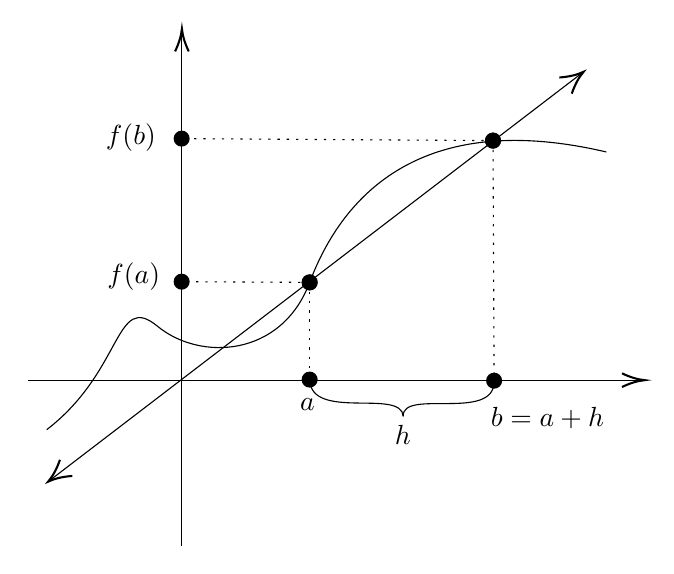
\begin{tikzpicture}[x=0.75pt,y=0.75pt,yscale=-1,xscale=1]
%uncomment if require: \path (0,441); %set diagram left start at 0, and has height of 441

%Straight Lines [id:da16102953695521127]
\draw    (163,221.33) -- (458,221.33) ;
\draw [shift={(460,221.33)}, rotate = 180] [color={rgb, 255:red, 0; green, 0; blue, 0 }  ][line width=0.75]    (10.93,-3.29) .. controls (6.95,-1.4) and (3.31,-0.3) .. (0,0) .. controls (3.31,0.3) and (6.95,1.4) .. (10.93,3.29)   ;
%Straight Lines [id:da9043079513680581]
\draw    (237.04,301) -- (237.04,54) ;
\draw [shift={(237.04,52)}, rotate = 90] [color={rgb, 255:red, 0; green, 0; blue, 0 }  ][line width=0.75]    (10.93,-3.29) .. controls (6.95,-1.4) and (3.31,-0.3) .. (0,0) .. controls (3.31,0.3) and (6.95,1.4) .. (10.93,3.29)   ;
%Curve Lines [id:da7565789477512073]
\draw    (171.9,245.19) .. controls (209.02,216.63) and (204.74,178.41) .. (225.27,195.34) .. controls (245.8,212.28) and (284.99,210.33) .. (298.59,174.22) .. controls (312.18,138.1) and (347.09,89.21) .. (441.52,111.39) ;
%Straight Lines [id:da9796385406474812]
\draw    (428.99,73.97) -- (174.17,269.02) ;
\draw [shift={(172.58,270.23)}, rotate = 322.57] [color={rgb, 255:red, 0; green, 0; blue, 0 }  ][line width=0.75]    (10.93,-4.9) .. controls (6.95,-2.3) and (3.31,-0.67) .. (0,0) .. controls (3.31,0.67) and (6.95,2.3) .. (10.93,4.9)   ;
\draw [shift={(430.57,72.75)}, rotate = 142.57] [color={rgb, 255:red, 0; green, 0; blue, 0 }  ][line width=0.75]    (10.93,-4.9) .. controls (6.95,-2.3) and (3.31,-0.67) .. (0,0) .. controls (3.31,0.67) and (6.95,2.3) .. (10.93,4.9)   ;
%Straight Lines [id:da4030910320179846]
\draw  [dash pattern={on 0.84pt off 2.51pt}]  (298.59,174.22) -- (298.59,221.05) ;
\draw [shift={(298.59,221.05)}, rotate = 90] [color={rgb, 255:red, 0; green, 0; blue, 0 }  ][fill={rgb, 255:red, 0; green, 0; blue, 0 }  ][line width=0.75]      (0, 0) circle [x radius= 3.35, y radius= 3.35]   ;
\draw [shift={(298.59,174.22)}, rotate = 90] [color={rgb, 255:red, 0; green, 0; blue, 0 }  ][fill={rgb, 255:red, 0; green, 0; blue, 0 }  ][line width=0.75]      (0, 0) circle [x radius= 3.35, y radius= 3.35]   ;
%Straight Lines [id:da14103701021608472]
\draw  [dash pattern={on 0.84pt off 2.51pt}]  (386.93,105.91) -- (387.46,221.58) ;
\draw [shift={(387.46,221.58)}, rotate = 89.74] [color={rgb, 255:red, 0; green, 0; blue, 0 }  ][fill={rgb, 255:red, 0; green, 0; blue, 0 }  ][line width=0.75]      (0, 0) circle [x radius= 3.35, y radius= 3.35]   ;
\draw [shift={(386.93,105.91)}, rotate = 89.74] [color={rgb, 255:red, 0; green, 0; blue, 0 }  ][fill={rgb, 255:red, 0; green, 0; blue, 0 }  ][line width=0.75]      (0, 0) circle [x radius= 3.35, y radius= 3.35]   ;
%Curve Lines [id:da47143485860977985]
\draw    (298.59,221.05) .. controls (299.18,241.14) and (342.98,225.16) .. (343.66,238.75) ;
%Curve Lines [id:da42610723931770456]
\draw    (387.46,221.58) .. controls (388.06,241.67) and (342.98,225.16) .. (343.66,238.75) ;
%Straight Lines [id:da3483526368480112]
\draw  [dash pattern={on 0.84pt off 2.51pt}]  (298.59,174.22) -- (236.91,173.88) ;
\draw [shift={(236.91,173.88)}, rotate = 180.32] [color={rgb, 255:red, 0; green, 0; blue, 0 }  ][fill={rgb, 255:red, 0; green, 0; blue, 0 }  ][line width=0.75]      (0, 0) circle [x radius= 3.35, y radius= 3.35]   ;
\draw [shift={(298.59,174.22)}, rotate = 180.32] [color={rgb, 255:red, 0; green, 0; blue, 0 }  ][fill={rgb, 255:red, 0; green, 0; blue, 0 }  ][line width=0.75]      (0, 0) circle [x radius= 3.35, y radius= 3.35]   ;
%Straight Lines [id:da4035786093366658]
\draw  [dash pattern={on 0.84pt off 2.51pt}]  (386.93,105.91) -- (236.91,104.95) ;
\draw [shift={(236.91,104.95)}, rotate = 180.37] [color={rgb, 255:red, 0; green, 0; blue, 0 }  ][fill={rgb, 255:red, 0; green, 0; blue, 0 }  ][line width=0.75]      (0, 0) circle [x radius= 3.35, y radius= 3.35]   ;
\draw [shift={(386.93,105.91)}, rotate = 180.37] [color={rgb, 255:red, 0; green, 0; blue, 0 }  ][fill={rgb, 255:red, 0; green, 0; blue, 0 }  ][line width=0.75]      (0, 0) circle [x radius= 3.35, y radius= 3.35]   ;

% Text Node
\draw (292.79,228.73) node [anchor=north west][inner sep=0.75pt]    {$a$};
% Text Node
\draw (384.59,233.05) node [anchor=north west][inner sep=0.75pt]    {$b=a+h$};
% Text Node
\draw (338.35,242.02) node [anchor=north west][inner sep=0.75pt]    {$h$};
% Text Node
\draw (199.88,163.44) node [anchor=north west][inner sep=0.75pt]    {$f( a)$};
% Text Node
\draw (199.19,96.46) node [anchor=north west][inner sep=0.75pt]    {$f( b)$};


\end{tikzpicture}

}

\vspace{4em}

\resizebox{3.25in}{!}{

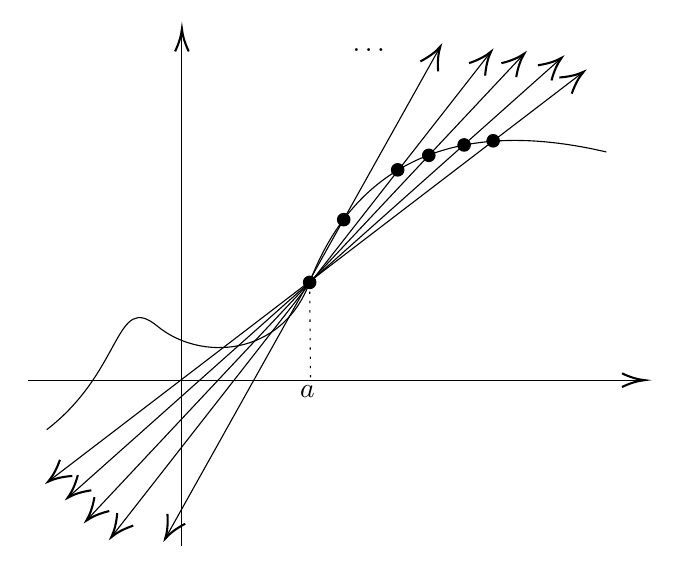
\begin{tikzpicture}[x=0.75pt,y=0.75pt,yscale=-1,xscale=1]
%uncomment if require: \path (0,441); %set diagram left start at 0, and has height of 441

%Straight Lines [id:da16102953695521127]
\draw    (163,221.33) -- (458,221.33) ;
\draw [shift={(460,221.33)}, rotate = 180] [color={rgb, 255:red, 0; green, 0; blue, 0 }  ][line width=0.75]    (10.93,-3.29) .. controls (6.95,-1.4) and (3.31,-0.3) .. (0,0) .. controls (3.31,0.3) and (6.95,1.4) .. (10.93,3.29)   ;
%Straight Lines [id:da9043079513680581]
\draw    (237.04,301) -- (237.04,54) ;
\draw [shift={(237.04,52)}, rotate = 90] [color={rgb, 255:red, 0; green, 0; blue, 0 }  ][line width=0.75]    (10.93,-3.29) .. controls (6.95,-1.4) and (3.31,-0.3) .. (0,0) .. controls (3.31,0.3) and (6.95,1.4) .. (10.93,3.29)   ;
%Curve Lines [id:da7565789477512073]
\draw    (171.9,245.19) .. controls (209.02,216.63) and (204.74,178.41) .. (225.27,195.34) .. controls (245.8,212.28) and (284.99,210.33) .. (298.59,174.22) .. controls (312.18,138.1) and (347.09,89.21) .. (441.52,111.39) ;
%Straight Lines [id:da9796385406474812]
\draw    (428.99,73.97) -- (174.17,269.02) ;
\draw [shift={(172.58,270.23)}, rotate = 322.57] [color={rgb, 255:red, 0; green, 0; blue, 0 }  ][line width=0.75]    (10.93,-4.9) .. controls (6.95,-2.3) and (3.31,-0.67) .. (0,0) .. controls (3.31,0.67) and (6.95,2.3) .. (10.93,4.9)   ;
\draw [shift={(430.57,72.75)}, rotate = 142.57] [color={rgb, 255:red, 0; green, 0; blue, 0 }  ][line width=0.75]    (10.93,-4.9) .. controls (6.95,-2.3) and (3.31,-0.67) .. (0,0) .. controls (3.31,0.67) and (6.95,2.3) .. (10.93,4.9)   ;
%Straight Lines [id:da1158565706067487]
\draw    (384.77,64.58) -- (204.23,295.42) ;
\draw [shift={(203,297)}, rotate = 308.03] [color={rgb, 255:red, 0; green, 0; blue, 0 }  ][line width=0.75]    (10.93,-4.9) .. controls (6.95,-2.3) and (3.31,-0.67) .. (0,0) .. controls (3.31,0.67) and (6.95,2.3) .. (10.93,4.9)   ;
\draw [shift={(386,63)}, rotate = 128.03] [color={rgb, 255:red, 0; green, 0; blue, 0 }  ][line width=0.75]    (10.93,-4.9) .. controls (6.95,-2.3) and (3.31,-0.67) .. (0,0) .. controls (3.31,0.67) and (6.95,2.3) .. (10.93,4.9)   ;
%Straight Lines [id:da7715304094905251]
\draw    (400.63,65.46) -- (192.37,287.54) ;
\draw [shift={(191,289)}, rotate = 313.16] [color={rgb, 255:red, 0; green, 0; blue, 0 }  ][line width=0.75]    (10.93,-4.9) .. controls (6.95,-2.3) and (3.31,-0.67) .. (0,0) .. controls (3.31,0.67) and (6.95,2.3) .. (10.93,4.9)   ;
\draw [shift={(402,64)}, rotate = 133.16] [color={rgb, 255:red, 0; green, 0; blue, 0 }  ][line width=0.75]    (10.93,-4.9) .. controls (6.95,-2.3) and (3.31,-0.67) .. (0,0) .. controls (3.31,0.67) and (6.95,2.3) .. (10.93,4.9)   ;
%Straight Lines [id:da44730990962603356]
\draw    (418.51,67.33) -- (183.49,276.67) ;
\draw [shift={(182,278)}, rotate = 318.31] [color={rgb, 255:red, 0; green, 0; blue, 0 }  ][line width=0.75]    (10.93,-4.9) .. controls (6.95,-2.3) and (3.31,-0.67) .. (0,0) .. controls (3.31,0.67) and (6.95,2.3) .. (10.93,4.9)   ;
\draw [shift={(420,66)}, rotate = 138.31] [color={rgb, 255:red, 0; green, 0; blue, 0 }  ][line width=0.75]    (10.93,-4.9) .. controls (6.95,-2.3) and (3.31,-0.67) .. (0,0) .. controls (3.31,0.67) and (6.95,2.3) .. (10.93,4.9)   ;
%Shape: Circle [id:dp8153494409622872]
\draw  [fill={rgb, 255:red, 0; green, 0; blue, 0 }  ,fill opacity=1 ] (384,106) .. controls (384,104.34) and (385.34,103) .. (387,103) .. controls (388.66,103) and (390,104.34) .. (390,106) .. controls (390,107.66) and (388.66,109) .. (387,109) .. controls (385.34,109) and (384,107.66) .. (384,106) -- cycle ;
%Shape: Circle [id:dp46038093787284295]
\draw  [fill={rgb, 255:red, 0; green, 0; blue, 0 }  ,fill opacity=1 ] (370,108) .. controls (370,106.34) and (371.34,105) .. (373,105) .. controls (374.66,105) and (376,106.34) .. (376,108) .. controls (376,109.66) and (374.66,111) .. (373,111) .. controls (371.34,111) and (370,109.66) .. (370,108) -- cycle ;
%Shape: Circle [id:dp190859565625209]
\draw  [fill={rgb, 255:red, 0; green, 0; blue, 0 }  ,fill opacity=1 ] (353,113) .. controls (353,111.34) and (354.34,110) .. (356,110) .. controls (357.66,110) and (359,111.34) .. (359,113) .. controls (359,114.66) and (357.66,116) .. (356,116) .. controls (354.34,116) and (353,114.66) .. (353,113) -- cycle ;
%Shape: Circle [id:dp3044800797092422]
\draw  [fill={rgb, 255:red, 0; green, 0; blue, 0 }  ,fill opacity=1 ] (338,120) .. controls (338,118.34) and (339.34,117) .. (341,117) .. controls (342.66,117) and (344,118.34) .. (344,120) .. controls (344,121.66) and (342.66,123) .. (341,123) .. controls (339.34,123) and (338,121.66) .. (338,120) -- cycle ;
%Shape: Circle [id:dp7651386739199335]
\draw  [fill={rgb, 255:red, 0; green, 0; blue, 0 }  ,fill opacity=1 ] (295.59,174.22) .. controls (295.59,172.56) and (296.93,171.22) .. (298.59,171.22) .. controls (300.24,171.22) and (301.59,172.56) .. (301.59,174.22) .. controls (301.59,175.87) and (300.24,177.22) .. (298.59,177.22) .. controls (296.93,177.22) and (295.59,175.87) .. (295.59,174.22) -- cycle ;
%Straight Lines [id:da21925282533113744]
\draw  [dash pattern={on 0.84pt off 2.51pt}]  (298.59,174.22) -- (299,221) ;
%Straight Lines [id:da4492754198498514]
\draw    (360.57,62.35) -- (229.98,295.92) ;
\draw [shift={(229,297.67)}, rotate = 299.21] [color={rgb, 255:red, 0; green, 0; blue, 0 }  ][line width=0.75]    (10.93,-4.9) .. controls (6.95,-2.3) and (3.31,-0.67) .. (0,0) .. controls (3.31,0.67) and (6.95,2.3) .. (10.93,4.9)   ;
\draw [shift={(361.54,60.61)}, rotate = 119.21] [color={rgb, 255:red, 0; green, 0; blue, 0 }  ][line width=0.75]    (10.93,-4.9) .. controls (6.95,-2.3) and (3.31,-0.67) .. (0,0) .. controls (3.31,0.67) and (6.95,2.3) .. (10.93,4.9)   ;
%Shape: Circle [id:dp18797969215530874]
\draw  [fill={rgb, 255:red, 0; green, 0; blue, 0 }  ,fill opacity=1 ] (312,144) .. controls (312,142.34) and (313.34,141) .. (315,141) .. controls (316.66,141) and (318,142.34) .. (318,144) .. controls (318,145.66) and (316.66,147) .. (315,147) .. controls (313.34,147) and (312,145.66) .. (312,144) -- cycle ;

% Text Node
\draw (292.79,222.73) node [anchor=north west][inner sep=0.75pt]    {$a$};
% Text Node
\draw (318,60.4) node [anchor=north west][inner sep=0.75pt]    {$\dotsc $};


\end{tikzpicture}

}

\end{multicols}


You'll notice that the tangent line captures some \textit{local information} about $f$ at $a$. In other words, it is a good approximation of $f$ at $a$; that is, $f$ and its tangent line are ``similar'' at $a$. Intuitively, you should think about the tangent line at $a$ to be the line that ``hugs $f$ the best at $a$.''

Note that this definition of the derivative only makes sense if $f$ is defined on an open interval containing $a$. We can view the derivative as a function, and write $[f(x)]'$ or $f'(x)$. The derivative of $f'(x)$ is called the \textbf{second derivative} and is denoted $f''(x)$. In general, the $n$th derivative $f^{(n)}(x)$ is defined to be the derivative of $f^{(n-1)}(x)$.

\subsection{The Two Part ``Program'' for Finding Derivatives}

So now we have a goal: find derivatives of functions. The problem is that the limit definition is difficult to use (that pesky $h\to 0$ in the denominator). So instead, we will do the following two steps (let $a$ be a real number and $f$ and $g$ be functions):
\begin{enumerate}
\item rules to break functions up and reassemble

\begin{center}
\def\arraystretch{1.5}
\begin{tabular}{@{}ll@{}}
\toprule[0.4mm]
\textbf{The Scalar Multiple Rule} & $[af]' = af'$. \\
\textbf{The Sum Rule} & $[f + g]' = f' + g'$ \\
\textbf{The Product Rule} & $[fg]' = f'g + fg'$ \\
\textbf{The Quotient Rule} & $\left[\frac{f}{g}\right]' = \frac{f'g - fg'}{g^2}$ \\
\textbf{The Chain Rule} & $[f(g(x))]' = f'(g(x))g'(x)$ \\
\textbf{The Inverse Rule} & $[f^{-1}(x)]' = \frac{1}{f'(f^{-1}(x))}$ \\
\bottomrule[0.4mm]
\end{tabular}
\end{center}

\item find derivatives of ``basic'' functions:

\end{enumerate}


\begin{center}
\def\arraystretch{1.5}
\begin{tabular}{@{}ll@{}}
\toprule[0.4mm]
\textbf{The Constant Rule}     & $[a]' = 0$ \\
\textbf{The Power Rule}        & $[x^a]' = ax^{a-1}$ \\
\textbf{Trig Rules}  & $[\sin(x)]' = \cos(x)$ and $[\cos(x)]' = -\sin(x)$ \\
\textbf{Exponential Rules} & $[a^x]' = \ln(a)a^x$ \\
\textbf{Logarithmic Rules} & $[\log_a(x)]' = \frac{1}{x\ln(a)}$ \\
\bottomrule[0.4mm]
\end{tabular}
\end{center}


Most of the time, you will be able to find the derivatives using a combination of these rules. For instance, the derivatives of the other 4 trig functions can be found using the quotient rule and the derivatives of $\sin$ and $\cos$:
$$[\tan(x)]' = \sec^2(x)
\quad\quad\quad\quad\quad
[\sec(x)]' = \sec(x)\tan(x)$$

$$[\cot(x)]' = -\csc^2(x)
\quad\quad\quad\quad\quad
[\csc(x)]' = -\csc(x)\cot(x)$$
\mar{See if you can find the pattern with these four derivatives. Hint: ``pSST''}


\subsection{Implicit Differentiation}

We'll refer to the set of points that satisfy an equation of two variables as a \textbf{curve in the plane}. Some examples you might have seen before are circles and ellipses. The circle with center $(h,k)$ and radius $r$ is the set of points $(x,y)$ in the plane that satisfy the equation
$$(x-h)^2+(y-k)^2=r^2.$$
\mar{Look up the similar equation for an ellipse.}

In general, curves are not functions (they might not pass the vertical line test), but they can have still have tangent lines, so we should be able to describe their slope at a point. We do this by ``zooming in'' on a point of the curve, and forgetting about the other parts of the curve. Now (locally), it looks like a function, so we can treat the $y$ variable as a function of $x$. This process is called ``implicit'' differentiation, and consists of two steps:
\begin{enumerate}
\item differentiate both sides of the equation (keeping in mind that since $y$ is a function of $x$, the derivative of $f(y)$ is $f'(y)\cdot y'$ by the chain rule).
\item solve for $y'$.
\end{enumerate}

Other notation is sometimes used: if $y=f(x)$, $\frac{dy}{dx}=\frac{d}{dx}[f(x)]$ is the derivative of $f$, and $\frac{d^ny}{dx^n}=\frac{d^n}{dx^n}[f(x)]$ is the $n$th derivative of $f$.

When you solve for $y'$, it is possible that the expression will consist of both $y$ and $x$ variables. That is because the formula for $y'$ is not a function of just $x$, it is a function of both $x$ and $y$!

Let's do an example:
\begin{itemize}
\item The curve of points satisfying the equation $y^{3}=x^{2}-xy-1$ is not a function, since it does not pass the vertical line test: both $(-1,-1)$ and $(-1,1)$ are solutions. However, we can still find the derivative at each point on this curve! Start by taking the ($x$) derivative of both sides.

On the left, the $x$ derivative of $y^3$ is $3y^2y'$, by the power rule (and the chain rule). The derivative of $x^2$ is $2x$, the derivative of $xy$ is $y+xy'$ by the product rule (and chain rule), and the derivative of $1$ is 0, of course. Comparing the derivatives of each side of the equation, we get
$$3y^2y'=2x-(y+xy'),$$
so solving for $y'$,
$$y'=\frac{2x-y}{3y^2+x}.$$
At $(-1,1)$, $y'=\frac{-3}{2}$, and at $(-1,-1)$, $y'=\frac{-1}{2}$. The tangent line to the curve at the point $(-1,1)$ is $y=\frac{-3}{2}(x+1)+1$

\end{itemize}


\subsection{Logarithmic Differentiation}

Sometimes you will be faced with a function whose formula includes an expression involving $x$ raised to a power that also involves $x$. Finding the derivative of such a function has a specific procedure: suppose $y=f(x)^{g(x)}$ and we want to find $y'$. First apply the $\ln$ function to both sides of the equation and use the log property $\ln(a^b)=b\ln(a)$:
$$\ln(y)=\ln(f(x)^{g(x)})=g(x)\ln(f(x)).$$
Then implicit differentiation yields
$$\frac{1}{y}y'=g'(x)\ln(f(x))+g(x)\frac{f'(x)}{f(x)},$$
and solving for $y'$ and substituting $y=f(x)^{g(x)}$ we get
$$y'=f(x)^{g(x)}\left(g'(x)\ln(f(x))+g(x)\frac{f'(x)}{f(x)}\right).$$
Here are some examples:
\begin{itemize}
\item $[x^x]'=x^x(\ln(x)+1)=\ln(x^{x^x})+x^x$. (Here $f(x)=g(x)=x$).
\item $[\sin(x)^x]'=\sin(x)^x(\ln(\sin(x))+x\cot(x))$. (Here $f(x)=\sin(x)$ and $g(x)=x$). \mar{Work these examples out.}
\end{itemize}

I don't recommend that you memorize the formula for $[f(x)^{g(x)}]'$. Instead, remember the procedure (called \textbf{Logarithmic Differentiation}) and re-create when you need it.


\subsection{Using The Inverse Rule}

When we want to find the derivative of an inverse of a function $f$, the inverse rule tells us that
$$[f^{-1}(x)]'=\frac{1}{f'(f^{-1}(x))},$$
but how is this helpful? It is actually very easy to see why this rule is true:
\begin{align*}
         & f(f^{-1}(x)) = x & & \text{(definition of inverse)}\\
\implies & f'(f^{-1}(x))[f^{-1}(x)]'=1 & &\text{(chain rule)}\\
\implies & [f^{-1}(x)]' = \frac{1}{f'(y)} & & \text{(solve for $[f^{-1}(x)]'$)}\\
\implies & [f^{-1}(x)]' =\frac{1}{f'(f^{-1}(x))} & & \text{(substitute)}
\end{align*}

Let's use this rule to find the derivative of inverse trig functions:
\begin{itemize}
\item The rule says that $[\sin^{-1}(x)]'=\frac{1}{\cos(\sin^{-1}(x))}$, but we should be able to simplify this expression using the unit circle.
\begin{figure}[h!]
\centering
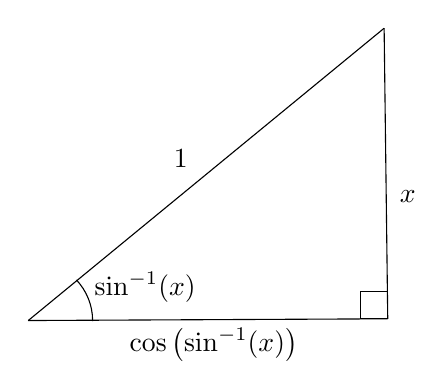
\begin{tikzpicture}[x=0.75pt,y=0.75pt,yscale=-1,xscale=1]
%uncomment if require: \path (0,479); %set diagram left start at 0, and has height of 479

%Straight Lines [id:da021711983663396772] 
\draw    (216.29,266.83) -- (389.5,266) ;
%Straight Lines [id:da1995895124000051] 
\draw    (387.76,126) -- (216.29,266.83) ;
%Shape: Arc [id:dp31180800912218465] 
\draw  [draw opacity=0] (239.51,247.26) .. controls (244.36,252.47) and (247.3,259.32) .. (247.3,266.83) .. controls (247.3,266.94) and (247.3,267.05) .. (247.3,267.16) -- (216.29,266.83) -- cycle ; \draw   (239.51,247.26) .. controls (244.36,252.47) and (247.3,259.32) .. (247.3,266.83) .. controls (247.3,266.94) and (247.3,267.05) .. (247.3,267.16) ;  
%Straight Lines [id:da12311387270862384] 
\draw    (387.76,126) -- (389.5,266) ;
%Shape: Square [id:dp5026691075905794] 
\draw   (376.5,253) -- (389.5,253) -- (389.5,266) -- (376.5,266) -- cycle ;

% Text Node
\draw (247,242) node [anchor=north west][inner sep=0.75pt]    {$\sin^{-1}( x)$};
% Text Node
\draw (263.9,269) node [anchor=north west][inner sep=0.75pt]   [align=left] {$\displaystyle \cos\left(\sin^{-1}(x)\right)$};
% Text Node
\draw (285.15,183.17) node [anchor=north west][inner sep=0.75pt]   [align=left] {$\displaystyle 1$};
% Text Node
\draw (394.13,203) node [anchor=north west][inner sep=0.75pt]   [align=left] {$\displaystyle x$};


\end{tikzpicture}
\end{figure}
if a (non-right) angle of a right triangle (with hypotenuse 1) is $\sin^{-1}(x)$, the leg opposite $\sin^{-1}(x)$ has length $x$. Then $\cos(\sin^{-1}(x))$ is the length of the other leg of the triangle, so $\cos(\sin^{-1}(x))=\sqrt{1-x^2}$ by the Pythagorean theorem. Therefore,
$$[\sin^{-1}(x)]'=\frac{1}{\cos(\sin^{-1}(x))}=\frac{1}{\sqrt{1-x^2}}.$$
\item The other derivatives of inverse trig functions are
$$[\cos^{-1}(x)]'=\frac{-1}{\sqrt{1-x^2}}$$
$$[\csc^{-1}(x)]'=\frac{-1}{|x|\sqrt{x^2-1}}\quad\quad [\sec^{-1}(x)]'=\frac{1}{|x|\sqrt{x^2-1}}$$
$$[\tan^{-1}(x)]'=\frac{1}{1+x^2}\quad\quad [\cot^{-1}(x)]'=\frac{1}{1+x^2}$$
\mar{Figure these equations out by yourself using the same method as for $\sin^{-1}$. Hint: refer to Figure \ref{6trig}}
\end{itemize}


\section{Applications}


\subsection{Linear Approximation}

This first application of derivatives is nothing too new! We first described the tangent line of a function $f$ as the line that ``hugs $f$ the best at $a$'' and now we are going to take of advantage of that fact.

The main idea is that if we have a function $f$ and we know $f(a)$ and $f'(a)$ for some $a$, then we can use the tangent line of $f$ at $a$ to estimate values of a function near $a$. That is, if $a\approx b$, then
$$f(b)\approx f(a)+f'(a)(b-a).$$\mar{When is this approximation an overestimate? Underestimate?}
The right side of this approximation is exactly the tangent line of $f$ at $a$, evaluated at $b$.

\begin{figure}[h!]
\centering
\fbox{
\tikzset{every picture/.style={line width=0.75pt}} %set default line width to 0.75pt
\begin{tikzpicture}[x=0.75pt,y=0.75pt,yscale=-1,xscale=1]
%uncomment if require: \path (0,300); %set diagram left start at 0, and has height of 300

%Straight Lines [id:da290856484859926] 
\draw    (189,231) -- (547,231.2) ;
%Straight Lines [id:da7357645784694884] 
\draw    (210,10) -- (210,272.2) ;
%Curve Lines [id:da5579528590630709] 
\draw    (210,231) .. controls (396,38) and (419,51) .. (540,226) ;
%Straight Lines [id:da4409257410178691] 
\draw    (205,170) -- (521,27.2) ;
%Straight Lines [id:da8838372850567859] 
\draw  [dash pattern={on 0.84pt off 2.51pt}]  (363,98.6) -- (363,232.2) ;
%Straight Lines [id:da5277023069496161] 
\draw  [dash pattern={on 0.84pt off 2.51pt}]  (407,79) -- (406,231) ;
%Straight Lines [id:da42915482489298684] 
\draw  [dash pattern={on 0.84pt off 2.51pt}]  (407,91.6) -- (210,93) ;
%Straight Lines [id:da3902230699344138] 
\draw  [dash pattern={on 0.84pt off 2.51pt}]  (407,79) -- (210.5,79) ;
%Straight Lines [id:da5116345937274027] 
\draw  [dash pattern={on 0.84pt off 2.51pt}]  (363,98.6) -- (210,100) ;
%Curve Lines [id:da33167985133818645] 
\draw    (169.75,48) .. controls (191.42,48) and (175.98,78.08) .. (208.96,78.98) ;
\draw [shift={(210.5,79)}, rotate = 180] [color={rgb, 255:red, 0; green, 0; blue, 0 }  ][line width=0.75]    (10.93,-3.29) .. controls (6.95,-1.4) and (3.31,-0.3) .. (0,0) .. controls (3.31,0.3) and (6.95,1.4) .. (10.93,3.29)   ;
%Curve Lines [id:da3661693241843025] 
\draw    (170.75,131) .. controls (193.16,131) and (175.55,100.92) .. (208.46,100.02) ;
\draw [shift={(210,100)}, rotate = 180] [color={rgb, 255:red, 0; green, 0; blue, 0 }  ][line width=0.75]    (10.93,-3.29) .. controls (6.95,-1.4) and (3.31,-0.3) .. (0,0) .. controls (3.31,0.3) and (6.95,1.4) .. (10.93,3.29)   ;
%Straight Lines [id:da2376462542003681] 
\draw    (170.75,93) -- (208,93) ;
\draw [shift={(210,93)}, rotate = 180] [color={rgb, 255:red, 0; green, 0; blue, 0 }  ][line width=0.75]    (10.93,-3.29) .. controls (6.95,-1.4) and (3.31,-0.3) .. (0,0) .. controls (3.31,0.3) and (6.95,1.4) .. (10.93,3.29)   ;

% Text Node
\draw (357,235) node [anchor=north west][inner sep=0.75pt]    {$a$};
% Text Node
\draw (137,120) node [anchor=north west][inner sep=0.75pt]    {$f(a)$};
% Text Node
\draw (401,235.4) node [anchor=north west][inner sep=0.75pt]    {$b$};
% Text Node
\draw (140,85) node [anchor=north west][inner sep=0.75pt]    {$f( b)$};
% Text Node
\draw (125,40) node [anchor=north west][inner sep=0.75pt]    {$\approx f( b)$};


\end{tikzpicture}
}
\caption{Linear Approximation}
\end{figure}

Let's pretend we don't have a calculator, and try to estimate $\sqrt{4.1}$. In this case $f(x)=\sqrt{x}$, and we should set $a=4$, since $4.1\approx 4$ and we can figure out $f(4)$ and $f'(4)$. By the power rule, $f'(x)=\frac{1}{2}x^{-1/2}$, so $f'(4)=\frac12(4^{-1/2})=\frac14$, and of course $f(4)=\sqrt{4}=2$. Using the formula above,
$$\sqrt{4.1}=f(4.1)\approx f(4)+f'(4)(4.1-4)=2+\frac14(0.1)=2.025.$$
If we check a calculator for a better approximation, we find that
$$\sqrt{4.1}\approx 2.02484567313,$$
so we weren't that far off! \mar{Estimate $\sqrt{3.9}$ and compare to the actual value.}

\subsection{L'H\^opital's Rule}

\textsc{In progress.}



\subsection{Comparing the Graphs of $f$, $f'$, and $f''$}
\textsc{In progress.}

% It is helpful to be able to look at a graph of a function and understand what it means for its first and second derivative. The table below summarizes:

% \begin{center}
% \def\arraystretch{1.3}
% \begin{tabular}{@{}lll@{}}
% \toprule[0.4mm]
% $f$ & $f'$ & $f''$ \\
% \midrule
% increasing & positive & \\
% constant & 0 & \\
% decreasing & negative & \\
% \midrule
% concave up & increasing & positive \\
% linear & constant & 0 \\
% concave down & decreasing & negative \\
% \bottomrule[0.4mm]

% Inflection point & constant & 0 \\ \hline
% local extrema & 0 & \\ \hline
% \hline

% \end{tabular}
% \end{center}


\subsection{Related Rates}
\textsc{In progress.}


\subsection{Optimization}
\textsc{In progress.}


\subsection{Newton's Method for Finding Roots}

Imagine that you have an function $f$ and you want to find the zeros (or roots) of $f$. That is, you want to find the values of $x$ such that $f(x)=0$. \textbf{Newton's Method} is a computational algorithm that can sometimes be used to approximate such a value. First, we'll describe the algorithm, and then we'll show how to do use your TI calculator to implement it.

Imagine that $x_0$ is an initial guess of a root of the function $f$. If we can take the derivative of $f$, then we know that the tangent line of $f$ at $x_0$ is
$$y-f(x_0)=f'(x_0)(x-x_0)$$
and so we find (setting $y=0$ and solving for $x$) this tangent line intersects the $x$-axis at the point $(x_1,0)$, where
$$x_1=x_0-\frac{f(x_0)}{f'(x_0)}.$$
We continue this, setting
$$x_2=x_1-\frac{f(x_1)}{f'(x_1)},$$
and so on:
$$x_{n+1}=x_n-\frac{f(x_n)}{f'(x_n)}.$$

In many cases, this sequence of numbers should approach a zero of $f$. Here is the intuitive reason why: (1) if $x_n$ is not a zero of $f$, then $x_{n+1}$ moves in the direction of a zero, and (2) if $x_n$ is a zero of $f$, then $x_{n+1}=x_n$.

The second point is obvious, but let's look into the first point. If $f(x_n)$ is not 0, then we have two cases:
\begin{itemize}
\item $x_{n+1}>x_n$ (move to the right).  Algebraically, this occurs exactly when $f(x_n)$ and $f'(x_n)$ have opposite sign (when $f$ is increasing below the $x$-axis, or decreasing above the $x$-axis).
\item $x_{n+1}<x_n$ (move to the left). Similarly, this occurs exactly when $f(x_n)$ and $f'(x_n)$ have the same sign (when $f$ is increasing above the $x$-axis, or decreasing below the $x$-axis).
\end{itemize}
\mar{Draw a picture showing the four cases.}
Seems reasonable, right? In either case we try to move in the direction of  a root.

Now, how do we use Newton's method? Get out your TI calculator, and type the function $f$ into \texttt{Y$_\text{1}$=}, and $f'$ into \texttt{Y$_\text{2}$=}. Then return to the main calculator screen and type
\begin{center}
\texttt{0 \MVRightarrow \ A}
\end{center}
(or replace the 0 with a different initial guess $x_0$) and click \texttt{ENTER}. Then type
\begin{center}
\texttt{A - Y$_\text{1}$(A)/Y$_\text{2}$(A) \MVRightarrow \ A}
\end{center}
and click \texttt{ENTER}. The variable \texttt{A} is now set as $x_1$, and this value should be displayed. Click \texttt{ENTER} again and \texttt{A} is now $x_2$. Continue clicking \texttt{ENTER} to find $x_n$ for higher $n$ (clicking 100 times will show you $x_{100}$).

Although Newton's method is generally an easy algorithm to implement and use, it does not always work.\mar{Consider $f(x)=x^3$ and try to use Newtons method to detect the root $0$ with the initial guess $x_0=1$.}




% \newpage
% \part{Anti-differentiation}
% \textsc{In Progress}







\end{document}












